%	PHẦN 1: CÁC PACKAGE CƠ BẢN VÀ CÁC TÙY CHỈNH VĂN BẢN
%----------------------------------------------------------------------------------------

\documentclass[
12pt,
oneside,
english,
doublespacing,
nolistspacing,
liststotoc,
parskip,
headsepline,
chapterinoneline,
]{HUSdissertation}

% \usepackage[utf8]{inputenc} 
\usepackage[utf8]{vietnam} 
%\usepackage[T1]{fontenc}

\usepackage{mathptmx}
\usepackage{amsmath}
\allowdisplaybreaks

%https://www.overleaf.com/learn/latex/Biblatex_citation_styles
%\usepackage[backend=bibtex,style=authoryear,natbib=true]{biblatex}
\usepackage[backend=bibtex,style=numeric,citestyle=ieee,natbib=true]{biblatex}

\addbibresource{main.bib}

\usepackage[autostyle=true]{csquotes}


%----------------------------------------------------------------------------------------
%	PHẦN 2: CÁC PACKAGE BỔ TRỢ THÊM VÀO TRONG QUÁ TRÌNH BIÊN SOẠN
%----------------------------------------------------------------------------------------

\RequirePackage{setlst}		% Liệt kê/trích dẫn code

\usepackage{multirow}
\usepackage{subfigure}
\usepackage[fontsize=13pt]{scrextend}

%https://www.sascha-frank.com/latex-font-size.html
%https://tex.stackexchange.com/questions/103286/how-to-change-section-subsection-font-size
\usepackage{titlesec}

\titleformat{\section}
{\normalfont\fontsize{13}{13}\bfseries}{\thesection}{1em}{}

\titleformat{\subsection}
{\normalfont\fontsize{13}{13}\bfseries\itshape}{\thesubsection}{1em}{}

%https://tex.stackexchange.com/questions/351961/how-to-indent-code-in-beginverbatim
\usepackage{fancyvrb} 		% Fancy Verbatim
\fvset{tabsize=4,vspace=0pt,fontsize=\footnotesize}

\usepackage{longtable} 		% Bảng dài - Long table

\usepackage[figuresright]{rotating} % Bảng ngang - Sideways table
\usepackage{tabularx}

\usepackage{fontawesome5} 	% Các biểu tượng, ký hiệu đặc biệt

\usepackage{tikz} 			% Vẽ hình
\usetikzlibrary{calc}

\usepackage{indentfirst}	% Lùi đầu dòng ở đầu đoạn văn
\setlength{\parindent}{0.5cm}

%----------------------------------------------------------------------------------------
%	PHẦN 3: THÔNG TIN VỀ Khóa luận tốt nghiệp/Tiểu luận (THESIS INFORMATION)
%----------------------------------------------------------------------------------------

\author{Lại Huy Hoàng \\ Nguyễn Trọng Tùng \\ Nguyễn Bá Tiến Phát \\ Tô Quang Hân} 
\thesistitle{Thiết kế và phát triển tác tử trí tuệ nhân tạo cho trò chơi Cờ Caro} 
\def\coursecode{NHẬP MÔN TRÍ TUỆ NHÂN TẠO (PHY1313)}
\supervisor {GS.TS. Nguyễn Thế Toàn}
\supervisorr{CN. Vi Anh Quân} 	% Tên này nếu không có thì để trống!

\field{Ngành Kỹ thuật điện tử và Tin học} 					% Ví dụ: "Ngành Vật lý", "Ngành Hóa học", v.v.
\doctype{Tiểu luận} 

\university{\href{http://hus.vnu.edu.vn}{Trường Đại học Khoa học Tự nhiên}}
\department{\href{http://hus.vnu.edu.vn/gioi-thieu/co-cau-to-chuc/khoa-truc-thuoc/khoa-vat-ly.html}{Khoa Vật lý}}

\AtBeginDocument{
	\hypersetup{pdftitle=\ttitle}
	\hypersetup{pdfauthor=\authorname}
}


\begin{document}
	
	\lstset{style=codeC}	% Thiết lập ngôn ngữ C/C++ là ngôn ngữ mặc định cho phần liệt kê souce code của cả bài
	
	\frontmatter 			% Sử dụng hệ thống đánh số La Mã (i, ii, iii, iv...) cho những trang trước phần mục lục
	
	\pagestyle{plain} 
	
	
	%----------------------------------------------------------------------------------------
	%	(KHÔNG CHỈNH SỬA PHẦN NÀY)
	%
	%	PHẦN 4: TRANG TIÊU ĐỀ/TRANG BÌA (TITLE PAGE)
	%----------------------------------------------------------------------------------------
	
	% TRANG BÌA CHÍNH:
	%----------------------------------------------------------------------------------------
%	(KHÔNG CHỈNH SỬA PHẦN NÀY)
%
%	Phần 6: TRANG TIÊU ĐỀ/TRANG BÌA (TITLE PAGE)
%----------------------------------------------------------------------------------------

% TRANG BÌA CHÍNH:
\begin{titlepage}
	\begin{tikzpicture}[overlay,remember picture]
		\draw [line width=3pt]
		($ (current page.north west) + (2.0cm,-2.0cm) $)
		rectangle
		($ (current page.south east) + (-1.5cm,1.8cm) $);
		\draw [line width=1pt]
		($ (current page.north west) + (2.15cm,-2.15cm) $)
		rectangle
		($ (current page.south east) + (-1.65cm,1.95cm) $); 
	\end{tikzpicture}
	\begin{center}
		
		\vspace{-.04\textheight}
		\noindent%\scshape
		\large \, \href{https://www.vnu.edu.vn/home/}{ĐẠI HỌC QUỐC GIA HÀ NỘI}\\
		\vspace{-0.25cm}{\large \MakeUppercase \univname}\\
		\vspace{-0.25cm}{\large \bfseries \MakeUppercase \deptname}\\[0.5cm]
		
\includegraphics{Logo/Logo_HUS_notext_nocolor}
		
		\vspace{1.0cm}
		
		{\large \MakeUppercase NHÓM 2}
		
		\vspace{2.5cm}
		
		{\Large \bfseries \MakeUppercase\ttitle\par}
		\vspace{0.4cm} % Khoảng cách từ tên đề tài xuống mã học phần
		{\large \bfseries NHẬP MÔN TRÍ TUỆ NHÂN TẠO (PHY1313)\par}
		
		\vspace{2.5cm}
		
		
		\vfill
		
		\textbf{Hà Nội - \the\year{}}
	\end{center}
\end{titlepage}


	
	% TRANG BÌA PHỤ:
	\include{sub-cover}
	
	
	%----------------------------------------------------------------------------------------
	%	PHẦN 5: DANH NGÔN (QUOTES)
	%----------------------------------------------------------------------------------------
	
	\vspace*{0.2\textheight}
	
	\noindent\enquote{\itshape 
		Không có đau đớn, sẽ không có bài học thực sự ý nghĩa.
	}\bigbreak
	
	\hfill Edward Elric (Fullmetal Alchemist: Brotherhood)
	
	
	%----------------------------------------------------------------------------------------
	%	PHẦN 6: LỜI CẢM ƠN (ACKNOWLEDGEMENTS)
	%----------------------------------------------------------------------------------------
	
	\begin{acknowledgements}
		\addchaptertocentry{\acknowledgementname}
		\thispagestyle{empty}
		
		\indent Lời đầu tiên, nhóm chúng em xin gửi lời cảm ơn chân thành và sâu sắc nhất đến các thầy cô giáo Trường Đại học Khoa học Tự nhiên, Đại học Quốc gia Hà Nội. Trong suốt quá trình học tập dưới mái trường, các thầy cô đã tận tình truyền dạy và trang bị cho nhóm những kiến thức nền tảng vô cùng quý báu, tạo tiền đề vững chắc để em thực hiện đề tài này.
		
		Bên cạnh đó, nhóm xin bày tỏ lòng biết ơn sâu sắc đến \textbf{TS. Nguyễn Thế Toàn} và \textbf{CN. Vi Anh Quân}, những người đã trực tiếp giảng dạy, chỉ bảo trong xuyên suốt môn học Nhập môn Trí tuệ nhân tạo. Sự hỗ trợ chuyên môn và những kiến thức bổ trợ quý báu về trí tuệ nhân tạo của hai thầy chính là kim chỉ nam giúp nhóm chúng em hoàn thiện đề tài. 
		
		Cuối cùng, xin cảm ơn tất cả các thành viên trong nhóm 2 đã luôn nỗ lực, đoàn kết và sẻ chia trách nhiệm. Mặc dù đã có nhiều cố gắng, song do kiến thức và kinh nghiệm lập trình thực tế còn hạn chế, quyển báo cáo khó tránh khỏi những thiếu sót. Nhóm rất mong nhận được những ý kiến đóng góp quý báu từ các thầy để đề tài có thể phát triển hoàn thiện hơn trong tương lai. 
		
		Nhóm tác giả xin chân thành cảm ơn!
		\begin{flushright}
			\itshape TP. Hà Nội, ngày 11 tháng 06 năm 2026 \\[0.2cm]
			\normalfont\bfseries Nhóm sinh viên thực hiện \\[0.2cm]
			\normalfont Nhóm 2
		\end{flushright}
		 
	\end{acknowledgements}
	
	
	%----------------------------------------------------------------------------------------
	%	(KHÔNG CHỈNH SỬA PHẦN NÀY)
	%
	%	PHẦN 7: MỤC LỤC (LIST OF CONTENTS/FIGURES/TABLES PAGES)
	%----------------------------------------------------------------------------------------
	
	\begin{spacing}{1.15}
		\tableofcontents 	% In ra mục lục chính
	\end{spacing}
	
	\begin{spacing}{1.15}
		\listoffigures 		% In ra danh sách hình vẽ
	\end{spacing}
	
	\begin{spacing}{1.15}
		\listoftables		% In ra danh sách bảng
	\end{spacing}
	
	
	%----------------------------------------------------------------------------------------
	%	PHẦN 8: DANH SÁCH TÊN VIẾT TẮT (ABBREVIATIONS)
	%----------------------------------------------------------------------------------------
	
	\begin{abbreviations}{ll} % Thêm danh sách tên viết tắt (dưới dạng một bảng có 2 cột)
		
		\textbf{AI}    & \textbf{A}rtificial \textbf{I}ntelligence (Trí tuệ nhân tạo) \\
		\textbf{API}   & \textbf{A}pplication \textbf{P}rogramming \textbf{I}nterface (Giao diện lập trình ứng dụng) \\
		\textbf{CPU}   & \textbf{C}entral \textbf{P}rocessing \textbf{U}nit (Bộ xử lý trung tâm) \\
		\textbf{GA}    & \textbf{G}enetic \textbf{A}lgorithm (Thuật toán di truyền) \\
		\textbf{GUI}   & \textbf{G}raphical \textbf{U}ser \textbf{I}nterface (Giao diện người dùng đồ họa) \\
		\textbf{MCTS}  & \textbf{M}onte \textbf{C}arlo \textbf{T}ree \textbf{S}earch (Tìm kiếm cây Monte Carlo) \\
		\textbf{PGN}   & \textbf{P}ortable \textbf{G}ame \textbf{N}otation (Biên bản ghi lại các nước đi trong trò chơi đối kháng) \\
		\textbf{RAM}   & \textbf{R}andom \textbf{A}ccess \textbf{M}emory (Bộ nhớ truy cập ngẫu nhiên) \\
		\textbf{SFX}   & \textbf{S}ound \textbf{F}e\textbf{x} (Hiệu ứng âm thanh đám đông/hành động) \\
		\textbf{TT}    & \textbf{T}ransposition \textbf{T}able (Bảng tra cứu trạng thái / Bảng chuyển vị) \\
		\textbf{UI}    & \textbf{U}ser \textbf{I}nterface (Giao diện người dùng) \\
		\textbf{UX}    & \textbf{U}ser \textbf{E}x\textbf{p}erience (Trải nghiệm người dùng) \\
	\end{abbreviations}
	
	
	%	%----------------------------------------------------------------------------------------
	%	%	PHẦN 9: CÁC HẰNG SỐ VẬT LÝ/THÔNG SỐ KĨ THUẬT (PHYSICAL CONSTANTS/OTHER DEFINITIONS)
	%	%----------------------------------------------------------------------------------------
	%	
	%	\begin{constants}{lr@{${}={}$}l} % Thêm danh sách các hằng số (dưới dạng một bảng có 3 cột)
		%		
		%		%	Lệnh \SI{}{} được cung cấp bởi gói siunitx, hãy đọc tài liệu hướng dẫn để biết cách sử dụng nó
		%		
		%		%	Tên hằng số 	 & $Biểu tượng$	& $Hằng số$ cùng với đơn vị\\
		%		Vận tốc ánh sáng & $c_{0}$		& \SI{2.99792458e8}{\meter\per\second} (chính xác)\\
		%		
		%	\end{constants}
	
	
	%----------------------------------------------------------------------------------------
	%	PHẦN 10: DANH SÁCH KÝ HIỆU (SYMBOLS)
	%----------------------------------------------------------------------------------------
	
	\begin{symbols}{lll} % Thêm danh sách các ký hiệu (dưới dạng một bảng có 3 cột)
		
		%   Ký hiệu	& Ý nghĩa		& Đơn vị \\
		$\mathbf{B}$     & Ma trận trạng thái bàn cờ hiện tại (kích thước $15 \times 15$ hoặc tùy chỉnh)\\
		$\mathbf{M}$     & Tập hợp các tọa độ nước đi tiềm năng được chọn lọc (interesting moves)\\
		$b$              & Hệ số nhánh (Branching factor) của cây quyết định\\
		$d$              & Độ sâu duyệt cây tối đa của thuật toán tìm kiếm (\texttt{bot\_depth})\\
		$H$              & Giá trị hàm lượng giá Heuristic tổng thể của một trạng thái bàn cờ\\
		
		\addlinespace % Khoảng cách để phân biệt giữa ký hiệu Latin với ký hiệu Hy Lạp
		
		$\alpha$         & Giá trị lượng giá tốt nhất (lớn nhất) mà người chơi Max chắc chắn đạt được\\
		$\beta$          & Giá trị lượng giá tốt nhất (nhỏ nhất) mà người chơi Min chắc chắn đạt được\\
		
	\end{symbols}
	
	
	%----------------------------------------------------------------------------------------
	%	(KHÔNG CHỈNH SỬA PHẦN NÀY)
	%
	%	PHẦN 11: LỜI ĐỀ TẶNG (DEDICATION)
	%----------------------------------------------------------------------------------------
	
	%\dedicatory{Dành tặng/Dành cho/Gửi tới\ldots} 
	
	
	%----------------------------------------------------------------------------------------
	%	PHẦN 12: NỘI DUNG/CÁC CHƯƠNG Khóa luận tốt nghiệp/Tiểu luận (THESIS CONTENT - CHAPTERS)
	%----------------------------------------------------------------------------------------
	
	\mainmatter % Bắt đầu đánh số trang (1,2,3...)
	
	\pagestyle{plain}
	
	% Hãy thêm những chương (chapter) của khóa luận/tiểu luận vào thư mục Chapters
	% Hãy bỏ chú thích những dòng nếu bạn đã bổ sung những chương vào
	
	% MỞ ĐẦU (LỜI MỞ ĐẦU - Chương 0)

\chapter*{MỞ ĐẦU} % Tên của chương
\addcontentsline{toc}{chapter}{MỞ ĐẦU} % Thêm tên chương vào mục lục

\label{Chapter0} % Để trích dẫn chương này ở chỗ nào đó trong bài, hãy sử dụng lệnh \ref{Chapter0} 

%----------------------------------------------------------------------------------------

Trong sự phát triển mạnh mẽ của khoa học máy tính, Trí tuệ nhân tạo đã và đang trở thành một lĩnh vực tiên phong, định hình lại cách con người tương tác với công nghệ. Trong bối cảnh đó, việc "số hóa" cờ Caro - một trò chơi dân gian quen thuộc của người Việt - không chỉ đáp ứng nhu cầu giải trí hiện đại mà còn tạo ra môi trường lý tưởng để thử nghiệm, đánh giá các thuật toán AI trong bài toán trò chơi đối kháng. 

Dù có luật chơi đơn giản, cờ Caro lại sở hữu không gian trạng thái khổng lồ. Đặc biệt, việc hệ thống cho phép tùy biến kích thước bàn cờ linh hoạt (10x10, 12x12 và lớn nhất là 15x15) khiến hệ số phân nhánh có thể lên tới 225, dẫn đến sự bùng nổ tổ hợp cực kỳ nhanh theo chiều sâu của cây quyết định. Việc tạo ra một tác tử AI có khả năng phân tích, lọc bỏ hàng triệu thế cờ vô giá trị để phản hồi thời gian thực với con người trên các kích thước bàn cờ khác nhau là một thử thách kỹ thuật lớn về mặt tối ưu thuật toán và quản lý tài nguyên máy tính.

Xuất phát từ những lý do trên, nhóm quyết định lựa chọn đề tài: \textbf{"Thiết kế và phát triển tác tử trí tuệ nhân tạo cho trò chơi Cờ Caro"}. 

\section*{Bố cục của tiểu luận}
Nội dung của tiểu luận gồm 5 chương chính như sau:
\begin{itemize}
	\item \textbf{Chương 1: Tổng quan đề tài:} Trình bày bối cảnh, lý do chọn đề tài, khảo sát các sản phẩm Caro AI hiện có và xác định bài toán cụ thể cần giải quyết.
	\item \textbf{Chương 2: Cơ sở lý thuyết:} Tập trung phân tích chuyên sâu lý thuyết về tìm kiếm đối kháng, chi tiết thuật toán Minimax, nguyên lý cắt tỉa Alpha-Beta và cách xây dựng hàm Heuristic cho cờ Caro.
	\item \textbf{Chương 3: Thiết kế và xây dựng hệ thống:} Chi tiết hóa kiến trúc phần mềm, cấu trúc dữ liệu ma trận bàn cờ, sơ đồ luồng dữ liệu, thuật toán giới hạn ô trống (Interesting Moves) và mã nguồn triển khai giao diện kết nối giữa các module do các thành viên thực hiện.
	\item \textbf{Chương 4: Kết quả thực nghiệm:} Đưa ra các số liệu thực tế thu thập được trong quá trình chạy thử nghiệm phần mềm về thời gian xử lý của AI ở các độ sâu (\textit{depth}) khác nhau, số lượng nút bị cắt tỉa và giao diện thực tế của chương trình khi vận hành.
	\item \textbf{Chương 5: Đánh giá và hướng phát triển:} Tổng kết các ưu điểm, hạn chế của hệ thống hiện tại, đánh giá hiệu quả làm việc nhóm và đề xuất các hướng cải tiến kỹ thuật như bảng chuyển vị (Transposition Table) hay học tăng cường trong tương lai.
\end{itemize}
	% Chương 1

\chapter{GIỚI THIỆU CHUNG} % Tên của chương

\label{Chapter1} % Để trích dẫn chương này ở chỗ nào đó trong bài, hãy sử dụng lệnh \ref{Chapter1} 

%----------------------------------------------------------------------------------------

% Định nghĩa một số lệnh cần thiết để điều chỉnh định dạng cho một số nội dung nhất định trong bài
\newcommand{\keyword}[1]{\textbf{#1}}
\newcommand{\tabhead}[1]{\textbf{#1}}
\newcommand{\code}[1]{\texttt{#1}}
\newcommand{\file}[1]{\texttt{\bfseries#1}}
\newcommand{\option}[1]{\texttt{\itshape#1}}

%----------------------------------------------------------------------------------------

\section{Giới thiệu về cờ Caro}
\subsection{Tổng quan về trò chơi}

Cờ Caro hay còn được biết đến rộng rãi với tên gọi Gomoku - một trò chơi cờ chiến thuật đối kháng có lịch sử lâu đời và có nguồn gốc từ châu Á. Trò chơi thường được cử hành trên một bàn cờ dạng lưới kẻ ô vuông với kích thước tiêu chuẩn là 15x15. Hai người chơi sẽ luân phiên đặt các quân cờ của mình (thường được ký hiệu trực quan là \textbf{X} và \textbf{O} trên máy tính, hoặc quân Đen và Trắng trong cờ vây) vào các giao điểm hoặc ô trống trên bàn cờ. Trận đấu sẽ chính thức kết thúc khi một trong hai người chơi tạo thành công một chuỗi liền mạch gồm đúng 5 quân cờ của mình theo một hướng bất kỳ: chiều ngang, chiều dọc hoặc đường chéo. 

Tại Việt Nam, cờ Caro không chỉ đơn thuần là một hình thức giải trí mà đã trở thành một nét văn hóa học đường độc đáo, một mảnh ghép ký ức gắn liền với biết bao thế hệ học sinh, sinh viên. Nhờ sự tối giản tuyệt đối về mặt công cụ - khi một ván cờ có thể bắt đầu ngay lập tức trên những trang vở giấy ô ly chỉ với hai chiếc bút - cờ Caro sở hữu khả năng tiếp cận cộng đồng sâu rộng. Tuy nhiên, đằng sau sự giản dị đó lại là một cuộc đấu trí đòi hỏi tư duy chiến thuật nhạy bén và khả năng tính toán sắc độ, tạo tiền đề vững chắc cho việc số hóa và phát triển trò chơi này thành các phần mềm máy tính hiện đại ngày nay.

Dưới góc độ Khoa học máy tính và Trí tuệ Nhân tạo, cờ Caro được phân loại là trò chơi đối kháng có thông tin hoàn hảo, mang tính xác định và có tổng bằng không (Deterministic, Perfect Information, Zero-Sum Game). Điều này đồng nghĩa với việc toàn bộ trạng thái của bàn cờ luôn được công khai minh bạch cho cả hai phe tại mọi thời điểm, không tồn tại bất kỳ yếu tố ngẫu nhiên hay may rủi nào (như việc đổ xúc xắc hay rút bài), và lợi ích của người chơi này chính là thiệt hại của người chơi kia. Những đặc trưng lý thuyết này khiến Caro trở thành một bài toán kinh điển và là môi trường thử nghiệm lý tưởng cho các mô hình, thuật toán tìm kiếm trên cây trò chơi.

\subsection{Luật chơi và điều kiện chiến thắng}

Để xây dựng một tác tử AI hoạt động chính xác, việc hệ thống hóa luật chơi là bước tiên quyết. Trò chơi cờ Caro trong đồ án này được thiết lập dựa trên các quy tắc truyền thống quen thuộc tại Việt Nam, bao gồm những điểm cốt lõi sau:

\begin{itemize}
	
	\item \textbf{Quy tắc bàn cờ và lượt đi:} Trận đấu diễn ra trên một bàn cờ lưới vuông (kích thước có thể tùy biến 10x10, 12x12 hoặc 15x15). Hai người chơi (hoặc một người và một AI) đại diện cho hai phe \textbf{X} và \textbf{O}. Bắt đầu ván cờ, bàn cờ hoàn toàn trống. Hai bên sẽ lần lượt luân phiên đánh dấu quân cờ của mình vào các ô trống chưa bị chiếm dụng.

	\item \textbf{Điều kiện chiến thắng cơ bản:} Mục tiêu cốt lõi của mỗi phe là cố gắng sắp xếp các quân cờ của mình tạo thành một chuỗi liền mạch gồm từ 5 quân cờ trở lên trên cùng một hàng ngang, hàng dọc hoặc đường chéo(luật chơi 5-in-a-row).

	\item \textbf{Biến thể "Luật chặn hai đầu" (Khóa đuôi):} Đây là luật chơi đặc trưng làm nên tính chiến thuật sâu sắc của cờ Caro Việt Nam so với luật Gomoku quốc tế tự do (Free Gomoku). Cụ thể, một chuỗi 5 quân cờ liên tiếp sẽ không được công nhận là chiến thắng nếu nó bị chặn đứng ở cả hai đầu bởi quân của đối phương (hoặc bị giới hạn bởi đường biên của bàn cờ). Để được phán quyết thắng cuộc, chuỗi 5 quân đó phải có ít nhất một đầu mở (tức là số lượng đầu bị chặn phải nhỏ hơn 2).

	\item \textbf{Luật hòa cờ (Draw):} Trận đấu sẽ được tuyên bố hòa khi toàn bộ các ô trống trên bàn cờ đều đã được đánh kín quân nhưng không có bất kỳ bên nào thiết lập được chuỗi chiến thắng hợp lệ.
	
\end{itemize}

Quy tắc "chặn hai đầu" mang ý nghĩa sống còn trong việc thiết kế \textbf{Hàm Heuristic} cho AI. Nó buộc hệ thống AI không chỉ rượt đuổi mục tiêu xếp đủ 5 quân, mà còn phải biết định lượng mức độ nguy hiểm của các thế cờ bị chặn để đưa ra quyết định phòng thủ kịp thời (ví dụ: sẵn sàng đánh một nước cờ chỉ để khóa đầu đối phương, biến chuỗi 4 quân mở 2 đầu thành chuỗi bị khóa chết).

\subsection{Thách thức kỹ thuật và bài toán bùng nổ tổ hợp}

Mặc dù quy tắc và luật chơi vô cùng dễ nắm bắt, độ phức tạp không gian trạng thái của cờ Caro lại vô cùng lớn, đặt ra những thử thách kỹ thuật không nhỏ cho quá trình phát triển tác tử thông minh:

\begin{itemize}
	\item \textbf{Sự bùng nổ tổ hợp:} Đối với một bàn cờ kích thước tiêu chuẩn 15x15, ngay ở nước đi đầu tiên, hệ số phân nhánh đã lên tới 225. Khi chiều sâu của cây quyết định tăng lên, số lượng trạng thái phải xét duyệt sẽ tăng trưởng theo hàm mũ, với không gian trạng thái tổng thể ước tính vượt quá ngưỡng $10^{105}$.
	
	\item \textbf{Sự bất khả thi của phương pháp vét cạn:} Sự bùng nổ tổ hợp khủng khiếp này biến việc duyệt toàn bộ cây trò chơi để tìm kiếm nước đi tối ưu tuyệt đối bằng phương pháp vét cạn (\textit{Brute-force}) trở nên hoàn toàn bất khả thi đối với năng lực phần cứng máy tính hiện tại trong giới hạn thời gian cho phép.
	
	\item \textbf{Yêu cầu đáp ứng thời gian thực (Real-time Constraint):} Để mang lại trải nghiệm thi đấu mượt mà cho con người, tác tử AI bắt buộc phải đưa ra quyết định phản hồi trong vòng vài giây. Việc cân bằng giữa độ sâu tìm kiếm (để AI đi nước cờ thông minh) và tốc độ xử lý là một bài toán hóc búa.
\end{itemize}

Do đó, bài toán đặt ra cho nhóm thực hiện đề tài là phải tìm cách thu hẹp không gian tìm kiếm một cách hiệu quả. Điều này đòi hỏi việc vận dụng linh hoạt thuật toán gốc Minimax, kết hợp chặt chẽ với kỹ thuật tối ưu hóa không gian duyệt Alpha-Beta Pruning để loại bỏ các nhánh yếu, đồng thời đề xuất các giải thuật giới hạn vùng nước đi trống và xây dựng hàm lượng giá Heuristic thông minh để định hướng cây quyết định.

\section{Mục tiêu của đề tài}

Mục tiêu cốt lõi của đề tài này là nghiên cứu, thiết kế và hiện thực hóa một hệ thống phần mềm trò chơi cờ Caro (10x10, 12x12, 15x15) hoàn chỉnh. Hệ thống không chỉ cung cấp giao diện tương tác trực quan mà quan trọng nhất là tích hợp một tác tử trí tuệ nhân tạo (Bot AI) có khả năng thi đấu đối kháng thời gian thực với con người hoặc đối kháng thực nghiệm giữa các tác tử với nhau. Để đạt được mục tiêu tổng thể đó, đề tài tập trung giải quyết các mục tiêu cụ thể sau:

\begin{itemize}
	\item \textbf{Triển khai thuật toán tìm kiếm đối kháng và đề xuất kỹ thuật tối ưu hóa giảm hệ số phân nhánh:} Hiện thực hóa thuật toán gốc Minimax kết hợp với kỹ thuật cắt tỉa Alpha-Beta (\textit{Alpha-Beta Pruning}) nhằm loại bỏ sớm các nhánh vô giá trị trên cây quyết định. Đặc biệt, để giải quyết thách thức bùng nổ tổ hợp do hệ số phân nhánh ban đầu quá lớn ($b = 225$), đề tài đề xuất và triển khai giải thuật tối ưu hóa vùng tìm kiếm. Kỹ thuật này giới hạn không gian nước đi tiềm năng trong một bán kính $R$ nhất định xung quanh các quân cờ hiện có, từ đó kéo giảm hệ số phân nhánh thực nghiệm xuống mức ổn định giúp thuật toán có khả năng duyệt sâu hơn trong thời gian thực.
	
	\item \textbf{Thiết kế hàm lượng giá Heuristic nhận diện mẫu hình chiến thuật:} Xây dựng một hàm lượng giá trạng thái bàn cờ ($H$) chuyên biệt cho biến thể cờ Caro 5-in-a-row. Hàm số này vận hành dựa trên cơ chế quét ma trận và đối chiếu mẫu hình để nhận diện và định giá các cấu trúc quân cờ chiến thuật (như chuỗi 4 quân mở hai đầu, chuỗi 3 quân đứt đoạn, chuỗi bị chặn). Điểm số tổng thể của trạng thái là hiệu số giữa thế trận tấn công (Attack Score) và thế trận phòng thủ (Defend Score), giúp Bot AI có tư duy nhạy bén trong việc cân bằng giữa tấn công chiếm thế thượng phong và phòng thủ ngăn chặn đối phương chiến thắng.
	
	\item \textbf{Chứng minh và đánh giá sự chênh lệch hiệu năng giữa lý thuyết và thực nghiệm:} Tiến hành thực nghiệm ghi lại dữ liệu vận hành của hệ thống dưới các cấu hình độ sâu khác nhau. Từ đó, thực hiện phân tích đối sánh, chứng minh bằng số liệu trực quan về sự chênh lệch hiệu năng (bao gồm tổng thời gian ra quyết định và số lượng nút thực tế phải duyệt trên cây) giữa công thức ước tính lý thuyết của cây quyết định vét cạn với số liệu thực tế sau khi đã áp dụng các kỹ thuật cắt tỉa Alpha-Beta và tối ưu vùng nước đi trống.
\end{itemize}

\section{Phạm vi nghiên cứu}

Để đảm bảo tính tập trung và độ khả thi của đề tài trong giới hạn tài nguyên tính toán của phần cứng thông dụng, phạm vi nghiên cứu được xác định cụ thể như sau:

\begin{itemize}
	\item \textbf{Không gian trạng thái và cấu trúc môi trường:} Nghiên cứu tập trung hoàn toàn vào môi trường bàn cờ lưới vuông kích thước cố định là $15 \times 15$ ô (tương đương với ma trận trạng thái có $225$ vị trí). Các thuật toán tối ưu hóa cấu trúc dữ liệu và tìm kiếm ô trống sẽ được thiết kế tối ưu hóa riêng cho không gian ma trận hai chiều này nhằm tránh lãng phí bộ nhớ RAM.
	
	\item \textbf{Quy tắc và luật chơi áp dụng:} Tác tử AI được lập trình để tuân thủ tuyệt đối luật cờ Caro 5-in-a-row. Điều kiện chiến thắng được phán quyết ngay khi một trong hai phe thiết lập được một chuỗi liền mạch từ 5 quân cờ trở lên theo hàng ngang, hàng dọc hoặc đường chéo. Các biến thể phức tạp khác của quốc tế (như luật Renju giới hạn nước đi mở đầu của quân Đen) nằm ngoài phạm vi xử lý của đề tài này.
	
	\item \textbf{Giới hạn độ sâu duyệt cây quyết định:} Nghiên cứu tập trung khảo sát và tìm ra ngưỡng độ sâu duyệt tối ưu cho hiệu năng tốt nhất - nơi cân bằng hoàn hảo giữa độ nhạy bén chiến thuật (AI không đi nước cờ thiển cận) và giới hạn thời gian phản hồi thời gian thực dưới 3 giây cho mỗi nước đi). Các cấu hình độ sâu vượt quá ngưỡng chịu tải của bộ vi xử lý đơn luồng CPU gây trễ phản hồi sẽ được ghi nhận như một giới hạn thực nghiệm thay vì mục tiêu ứng dụng thực tế.
\end{itemize}
	%----------------------------------------------------------------------------------------
%	CHƯƠNG 2: CƠ SỞ LÝ THUYẾT
%----------------------------------------------------------------------------------------

\chapter{CƠ SỞ LÝ THUYẾT}
\label{Chapter2}

% =================================================================
%   MỤC 2.1
% =================================================================
\section{Tìm kiếm đối kháng}
% Tiểu mục 2.1.1
\subsection{Lý thuyết trò chơi}

Trong lĩnh vực Trí tuệ nhân tạo, khi đối mặt với các môi trường đa tác tử, lý thuyết trò chơi cung cấp các góc nhìn hệ thống để mô hình hóa hành vi của đối thủ nhằm tìm ra quyết định tối ưu. Có ít nhất ba góc nhìn chiến lược mà hệ thống có thể lấy làm điểm xuất phát để phân tích hành vi:

\begin{itemize}
	\item \textbf{Góc nhìn kinh tế tổng hợp:} Góc nhìn này tiếp cận môi trường dưới dạng một nền kinh tế, cực kỳ phù hợp khi có một số lượng rất lớn các tác tử tham gia vĩ mô. Nó cho phép chúng ta dự đoán các xu hướng tổng hợp (ví dụ: nhu cầu tăng sẽ đẩy giá cả lên cao) mà không cần phải dự đoán chính xác hành động riêng lẻ của từng tác tử cụ thể. Hướng tiếp cận này được áp dụng rộng rãi trong các bài toán tối ưu nguồn lực phức tạp nhưng không phù hợp cho dạng đối kháng tay đôi.
	\item \textbf{Góc nhìn môi trường biến động ngẫu nhiên:} Góc nhìn này xem các tác tử đối kháng đơn thuần là một phần của môi trường động và biến nó thành một môi trường không xác định. Việc mô hình hóa đối thủ theo cách này tương tự như cách xử lý hiện tượng tự nhiên ngẫu nhiên (ví dụ: trời đôi khi mưa và đôi khi không). Cách tiếp cận này dẫu đơn giản nhưng lại bỏ sót một thực tế quan trọng: \textbf{đối thủ đang chủ động tìm mọi cách để đánh bại chúng ta}, trong khi các hiện tượng tự nhiên như mưa hoàn toàn không có ý định hay chiến lược cốt lõi đó.
	\item \textbf{Góc nhìn tìm kiếm cây trò chơi đối kháng:} Chúng ta tiến hành mô hình hóa một cách tường minh hành vi của đối thủ thông qua các kỹ thuật duyệt cây trò chơi nhằm tìm ra chiến lược phản đòn hợp lý nhất
\end{itemize}
Từ góc nhìn tìm kiếm đối kháng này, hệ thống sẽ đi qua một lớp trò chơi có điều kiện hạn chế như cờ Caro để định nghĩa thế nào là một nước đi tối ưu và áp dụng thuật toán \textbf{Tìm kiếm Minimax} làm nền tảng xử lý gốc. Giải thuật này giả định cả hai người chơi đều có lý trí và đưa ra các nước đi hoàn hảo để đối đầu nhau 
%-----------------------------------
%	TIỂU MỤC 2
%-----------------------------------

\subsection{Mô hình hóa cờ Caro bằng Cây trò chơi}

Trò chơi cờ caro được định nghĩa bao gồm các thành phần cốt lõi sau:
\begin{itemize}
	\item \textbf{$S_0$ (Root Node):} Là nút gốc cao nhất của cây trò chơi, biểu diễn trạng thái bàn cờ hoàn toàn trống rỗng khi ván đấu bắt đầu.
	
	\item \textbf{\texttt{TO-MOVE}(s):} Xác định danh tính người chơi có quyền thực hiện nước đi tại trạng thái hiện tại $s$. Trong mô hình đối kháng tay đôi này, quyền quyết định sẽ luân phiên tuần tự giữa hai tác tử: người chơi tối đa hóa lợi ích (MAX) và người chơi tối thiểu hóa lợi ích (MIN). 
	
	\item \textbf{\texttt{Actions}(s):} Trả về danh sách tất cả các nước đi hợp lệ mà một người chơi được phép thực hiện tại trạng thái $s$. Đối với cờ Caro, hành động này là việc đặt một quân cờ vào các vị trí ô lưới còn trống trên bàn cờ. Trong các cài đặt thực tế nhằm tối ưu hiệu năng duyệt cây, tập hợp hành động này thường được giới hạn thu hẹp trong phạm vi các ô trống xung quanh vùng đang có quân cờ để tránh duyệt các ô biệt lập vô nghĩa.
	
	\item \textbf{\texttt{Result}(s, a):} Mô hình chuyển dịch trạng thái, trả về một nút con mới trên cây sau khi hành động $a$ được thực thi thành công tại nút cha $s$. Do môi trường mang tính xác định cao, một cặp $(s, a)$ cố định luôn luôn dẫn đến một kết quả \texttt{Result}(s, a) duy nhất.
	
	\item \textbf{\texttt{IS-TERMINAL}(s):} Hàm logic thực hiện nhiệm vụ quét trạng thái bàn cờ để xác định ván cờ đã đạt đến điều kiện dừng hay chưa. Trận đấu sẽ dừng lại khi xuất hiện một chuỗi chiến thắng gồm đúng 5 quân cờ liên tiếp hợp lệ hoặc khi bàn cờ đã bị lấp đầy hoàn toàn dẫn đến cục diện hòa. Các nút thỏa mãn điều kiện dừng này được gọi là nút lá (Terminal Nodes) và không phát triển thêm nhánh con.
	
	\item \textbf{\texttt{Utility}(s, p):} Hàm lợi ích (còn được gọi là hàm mục tiêu hoặc hàm trả thưởng), xác định giá trị số cuối cùng cho người chơi $p$ khi trò chơi kết thúc ở trạng thái kết thúc $s$.
\end{itemize}

\begin{center}
	\nopagebreak
	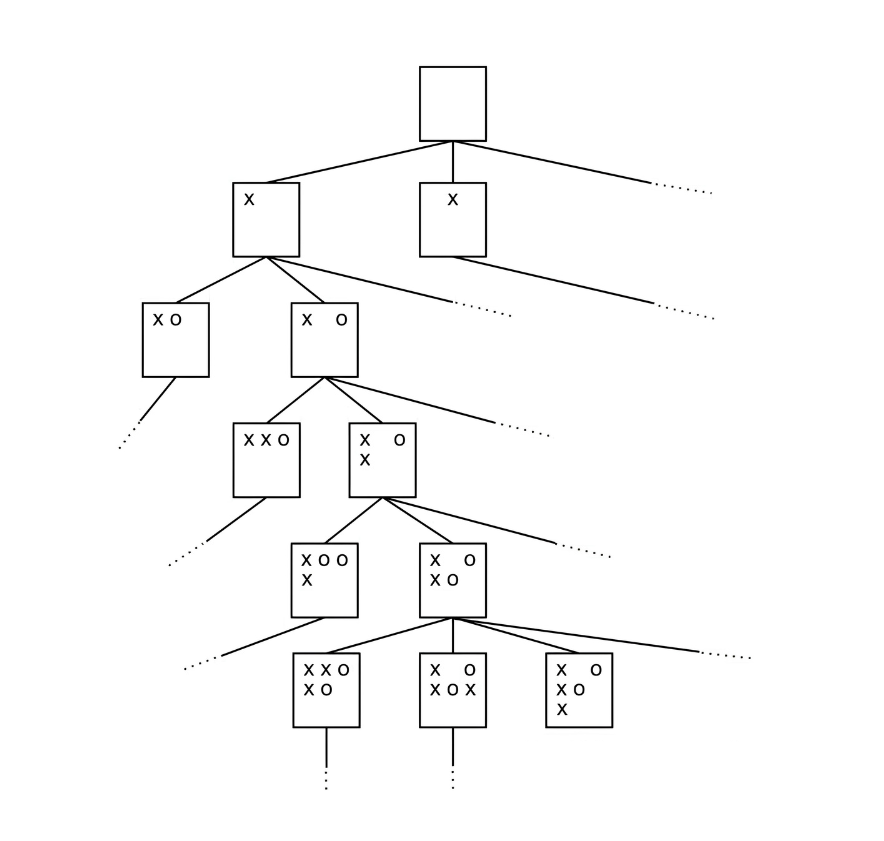
\includegraphics[width=0.55\textwidth]{Figures/Gallery/gametree.png}
	\captionof{figure}{Cây trò chơi của cờ Caro 3x3 (Tic-Tac-Toe)}
	\label{fig:game_tree}
\end{center}
\vspace{0.3cm}

Một tham số kỹ thuật cực kỳ quan trọng chi phối trực tiếp đến cấu trúc hình học và độ phình của cây trò chơi là hệ số phân nhánh $b$, đại diện cho số lượng nước đi hợp lệ trung bình tại mỗi tầng của cây. Đối với bàn cờ Caro tiêu chuẩn kích thước 15x15, ở nước cờ đầu tiên hệ số phân nhánh tối đa lên tới \textit{225} và giảm dần sau mỗi nước đi tiếp theo.
%----------------------------------------------------------------------------------------
%	MỤC 2
%----------------------------------------------------------------------------------------

\section{Thuật toán tìm kiếm Minimax}

Thuật toán Minimax là giải thuật nền tảng được thiết kế chuyên biệt để giải quyết các bài toán tìm kiếm đối kháng trong mô hình trò chơi có tổng bằng không (zero-sum games). Bản chất của đặc tính ``tổng bằng không'' quy định rằng bất kỳ một nước đi nào mang lại lợi thế cho một người chơi sẽ tương ứng mang lại một lượng thiệt hại hoặc hình phạt có giá trị tuyệt đối bằng chừng đó cho người chơi đối phương, nghĩa là cục diện ván cờ luôn được duy trì dưới dạng một cán cân toán học cân bằng và không tồn tại bất kỳ kết quả đôi bên cùng có lợi (win-win outcome) nào. Để vận hành mô hình này, giải thuật phân định hai thực thể tham gia luân phiên bằng tên gọi toán học là MAX (đại diện cho tác tử AI) và MIN (đại diện cho người chơi đối phương), trong đó hai người chơi sẽ thay phiên nhau đặt các quân cờ cho đến khi trận đấu đạt trạng thái kết thúc. Tại các nút lá kết thúc này, các giá trị số học cao sẽ đại diện cho phần thưởng tốt đối với góc nhìn chiến lược của tác tử MAX và đồng thời là kết quả tồi tệ nhất đối với góc nhìn của tác tử MIN.

Về bản chất vận hành, thuật toán Minimax là một chiến lược chơi game mạnh mẽ hoạt động trực tiếp trên cấu trúc cây trò chơi. Cơ chế cốt lõi của giải thuật là việc hình dung ra kịch bản xấu nhất có thể xảy ra từ bất kỳ nước đi nào của bản thân dưới sự phản công thông minh từ phía đối thủ, và sau đó chọn lựa nước đi dẫn đến kịch bản xấu nhất tốt nhất - tức là tìm kiếm giải pháp ``ít tệ nhất'' trong số các tình huống nguy hiểm có thể xảy ra. 

Thuật toán Minimax lựa chọn hành động tối ưu theo tiến trình các bước cụ thể sau:
\begin{enumerate}
	\item \textbf{Khởi tạo cây tìm kiếm giới hạn:} Xây dựng một cây trò chơi biểu diễn toàn bộ các trạng thái có thể mở rộng của trò chơi từ thời điểm hiện tại.
	\item \textbf{Xác định giá trị tại các nút lá giới hạn:} Xác định từng nút lá đại diện cho trạng thái cuối cùng (hoặc trạng thái dừng tại độ sâu giới hạn) và gán cho nó giá trị Minimax tùy thuộc vào việc nó tương ứng với kết quả thắng ($+1$), thua ($-1$) hoặc hòa ($0$) đối với tác tử.
	\item \textbf{Lan truyền ngược giá trị lên các nút cha:} Liên tục truyền các giá trị định lượng đó ngược lên cây để xác định giá trị cho các nút cha. Tiến trình này giả định bạn luôn cố gắng giành chiến thắng (tối đa hóa giá trị lợi ích) và đối thủ của bạn có lý trí sẽ luôn cố gắng khiến bạn thua (tối thiểu hóa giá trị lợi ích của bạn):
	\begin{itemize}
		
		\item \textbf{Nếu nút cha tương ứng với lượt đi của bạn (MAX):} Giá trị Minimax của nút cha sẽ bằng giá trị lớn nhất ($\max$) trong số các giá trị của các nút con trực tiếp, bởi vì bạn luôn muốn tối đa hóa lợi thế và điểm số của bản thân.
		
		\item \textbf{Nếu nút cha tương ứng với lượt đi của đối thủ (MIN):} Giá trị Minimax của nút cha sẽ bằng giá trị nhỏ nhất ($\min$) trong số các giá trị của các nút con trực tiếp, bởi vì hệ thống mặc định đối thủ có lý trí sẽ luôn muốn tối thiểu hóa điểm số để kìm hãm bạn.
	\end{itemize}
	\item \textbf{Ra quyết định nước đi tối ưu:} Tại nút gốc (trạng thái hiện tại của bàn cờ), tác tử AI sẽ luôn luôn lựa chọn hành động dẫn dắt trò chơi dịch chuyển sang nút con có giá trị Minimax cao nhất. Trong trường hợp xuất hiện nhiều nút con có giá trị tối ưu bằng nhau, hệ thống có thể phá vỡ thế cân bằng bằng cách lựa chọn ngẫu nhiên một trong các nước đi đó.
\end{enumerate}

 Mô hình toán học tổng quát chi phối toàn bộ tiến trình 4 bước nêu trên được thiết lập theo công thức đệ quy luân phiên sau:

 $$\text{MINIMAX}(s) = 
 \begin{cases} 
 	\text{UTILITY}(s, \text{MAX}) & \text{if } \text{IS-TERMINAL}(s) \\ 
 	\max_{a \in \text{Actions}(s)} \text{MINIMAX}(\text{RESULT}(s, a)) & \text{if } \text{TO-MOVE}(s) = \text{MAX} \\ 
 	\min_{a \in \text{Actions}(s)} \text{MINIMAX}(\text{RESULT}(s, a)) & \text{if } \text{TO-MOVE}(s) = \text{MIN} 
 \end{cases}$$
 \begin{center}
 	\nopagebreak
 	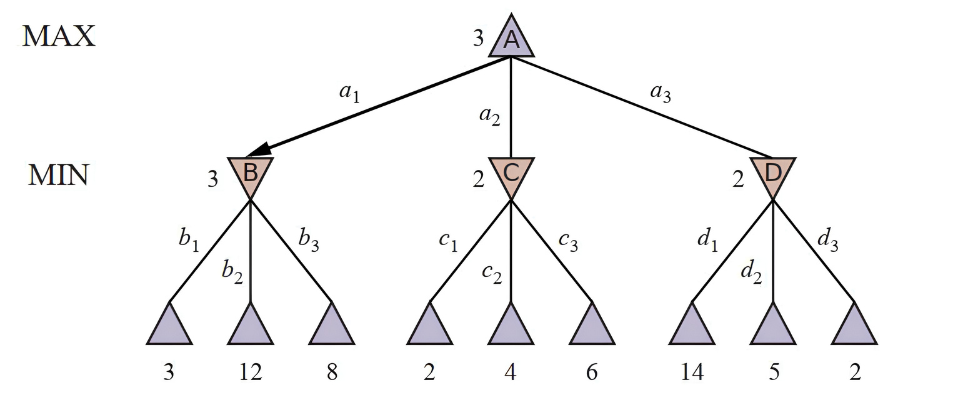
\includegraphics[width=\textwidth]{Figures/Gallery/minimax.png}
 	\captionof{figure}{Sơ đồ cây tìm kiếm đối kháng và tiến trình lan truyền ngược Minimax giữa hai tác tử MAX và MIN}
 	\label{fig:minimax}
 \end{center}
 \vspace{0.3cm}
 Mặc dù giải thuật đảm bảo tìm ra chiến lược tối ưu tuyệt đối, việc phải duyệt toàn bộ cây trò chơi đến tận các nút lá khiến tổng số lượng trạng thái cần tính toán tăng trưởng theo hàm mũ $b^d$. Do đó, độ phức tạp thời gian của thuật toán Minimax trong kịch bản xấu nhất là $\mathcal{O}(b^d)$, trong khi độ phức tạp không gian bộ nhớ lưu trữ các nút trên đường đi hiện tại là $\mathcal{O}(bd)$. 
 
 Đối với các trò chơi sở hữu không gian trạng thái rộng lớn như cờ Caro, sự bùng nổ tổ hợp này đặt ra thách thức cực kỳ lớn cho năng lực tính toán của phần cứng. 
 
 \begin{table}[!htbp]
 	\centering
 	\caption{Minh họa sự bùng nổ tổ hợp số nút cần duyệt theo độ sâu}
 	\label{tab:combinatorial_explosion}
 	\begin{tabular}{|c|c|c|r|}
 		\hline
 		\textbf{Bàn cờ} & \textbf{\textit{b}} & \textbf{\textit{d}} & \textbf{Số nút} \\ \hline
 		\multirow{3}{*}{10x10} & 100 & 1 & 100 \\ \cline{2-4} 
 		& 100 & 2 & 10.000 \\ \cline{2-4} 
 		& 100 & 3 & 1.000.000 \\ \hline
 		\multirow{3}{*}{12x12} & 144 & 1 & 144 \\ \cline{2-4} 
 		& 144 & 2 & 20.736 \\ \cline{2-4} 
 		& 144 & 3 & 2.985.984 \\ \hline
 		\multirow{3}{*}{15x15} & 225 & 1 & 225 \\ \cline{2-4} 
 		& 225 & 2 & 50.625 \\ \cline{2-4} 
 		& 225 & 3 & 11.390.625 \\ \hline
 	\end{tabular}
 \end{table}
 
Sự gia tăng nhanh chóng của số lượng trạng thái như dữ liệu thống kê trên chính là giới hạn vật lý kìm hãm chiều sâu tư duy của AI. Đây cũng là tiền đề cốt lõi thúc đẩy việc nghiên cứu và áp dụng các kỹ thuật cải tiến, tối ưu hóa thọc sâu trực tiếp vào cấu trúc cây trò chơi ở các mục tiếp theo nhằm cắt tỉa bớt các nhánh thừa vô nghĩa mà vẫn bảo toàn tính chính xác của quyết định.
 
\section{Thuật toán cắt tỉa $\alpha$ - $\beta$} 
Nhược điểm lớn nhất của thuật toán Minimax thuần túy là hiện tượng bùng nổ tổ hợp do phải duyệt qua toàn bộ các trạng thái trên cây trò chơi với độ phức tạp thời gian theo hàm mũ $\mathcal{O}(b^d)$, khiến việc tính toán trở nên bất khả thi đối với các trò chơi có hệ số phân nhánh lớn như cờ Caro. Để tối ưu hóa hiệu năng tính toán mà không làm thay đổi kết quả lựa chọn nước đi cuối cùng tại nút gốc, kỹ thuật \textbf{Cắt tỉa Alpha-Beta (Alpha-Beta Pruning)} được tích hợp trực tiếp vào tiến trình duyệt cây theo chiều sâu (DFS). Vì bản chất của Minimax là tìm kiếm theo chiều sâu, tại bất kỳ thời điểm nào, hệ thống chỉ cần xem xét các nút dọc theo một đường dẫn duy nhất trên cây trò chơi. 

Bản chất của kỹ thuật cắt tỉa này là bỏ qua việc đánh giá các nhánh của cây trò chơi mà hệ thống chứng minh được rằng chúng chắc chắn sẽ không ảnh hưởng đến quyết định của các tác tử có lý trí ở nút gốc. Phép cắt tỉa vận hành bằng cách duy trì hai tham số toán học xuyên suốt quá trình tìm kiếm: 
\begin{itemize}
	\item \textbf{Tham số $\alpha$ (Alpha):} Đại diện cho giá trị của sự lựa chọn tốt nhất (giá trị cao nhất) mà hệ thống đã tìm được cho đến thời điểm hiện tại tại bất kỳ điểm lựa chọn nào dọc theo đường đi của tác tử MAX. Về mặt toán học, $\alpha$ đóng vai trò là một ngưỡng chặn dưới (định nghĩa theo tư duy: ``ít nhất là'' - \textit{at least}).
	\item \textbf{Tham số $\beta$ (Beta):} Đại diện cho giá trị của sự lựa chọn tốt nhất (giá trị thấp nhất) mà hệ thống đã tìm được cho đến thời điểm hiện tại tại bất kỳ điểm lựa chọn nào dọc theo đường đi của tác tử MIN. Về mặt toán học, $\beta$ đóng vai trò là một ngưỡng chặn trên (định nghĩa theo tư duy: ``nhiều nhất là'' - \textit{at most}).
\end{itemize}

Thuật toán cắt tỉa Alpha-Beta thực hiện cập nhật liên tục hai tham số này thông qua một tiến trình xử lý liên tục: các giá trị $\alpha$ và $\beta$ hiện thời từ nút cha sẽ được truyền trực tiếp xuống cho các nút con tính toán khi đi sâu xuống cây trò chơi. Tại các nút thuộc lượt đi của MAX, hệ thống nhận các giá trị trả về từ các nút con và liên tục cập nhật tham số $\alpha$ bằng cách lấy giá trị lớn nhất ($\max$) giữa $\alpha$ hiện tại và giá trị của nút con vừa duyệt. Ngược lại, tại các nút thuộc lượt đi của MIN, hệ thống liên tục cập nhật tham số $\beta$ bằng cách lấy giá trị nhỏ nhất ($\min$) giữa $\beta$ hiện tại và giá trị của nút con vừa duyệt.

Tại bất kỳ thời điểm nào trong quá trình duyệt, nếu hệ thống phát hiện ra điều kiện toán học:
$$\alpha \ge \beta$$
Tiến trình cắt tỉa sẽ lập tức được kích hoạt để ngừng duyệt tất cả các nhánh con còn lại của nút hiện tại vì việc duyệt thêm trở nên hoàn toàn vô nghĩa. Phép cắt tỉa này được phân chia thành hai trường hợp cụ thể:

\begin{enumerate}
	\item \textbf{Cắt tỉa xảy ra tại một nút thuộc lượt của MIN (Alpha-cut):} 
	\begin{itemize}
		\item \textbf{Cơ chế:} Khi tác tử MIN tìm thấy một nước đi có giá trị nhỏ hơn hoặc bằng giá trị $\alpha$ hiện thời (ngưỡng chặn dưới mà MAX đã đảm bảo đạt được ở các nhánh trước).
		\item \textbf{Hệ quả:} Do tác tử MIN có lý trí chắc chắn sẽ ưu tiên chọn nước đi thấp hơn hoặc bằng này, nó sẽ khiến giá trị của toàn bộ nút MIN hiện tại không thể vượt qua $\alpha$. Kết quả là nút cha MAX ở tầng trên sẽ không bao giờ lựa chọn nhánh này nữa. Vì vậy, hệ thống lập tức dừng duyệt toàn bộ các nhánh con còn lại của nút MIN hiện tại.
	\end{itemize}
	
	\item \textbf{Cắt tỉa xảy ra tại một nút thuộc lượt của MAX (Beta-cut):} 
	\begin{itemize}
		\item \textbf{Cơ chế:} Khi tác tử MAX tìm thấy một nước đi có giá trị lớn hơn hoặc bằng giá trị $\beta$ hiện thời (ngưỡng chặn trên mà MIN giới hạn cho phép ở tầng trước).
		\item\textbf{Hệ quả:} Do tác tử MAX chắc chắn sẽ chọn nước đi cao hơn hoặc bằng này, nó làm cho giá trị của nút MAX hiện tại chắc chắn vượt qua ngưỡng $\beta$. Điều này dẫn đến việc nút cha MIN ở tầng trên sẽ loại bỏ ngay lập tức việc lựa chọn nhánh này. Vì vậy, tiến trình duyệt các nhánh con còn lại của nút MAX hiện hành lập tức bị bẻ gãy.
	\end{itemize}
\end{enumerate}
 \begin{center}
	\nopagebreak
	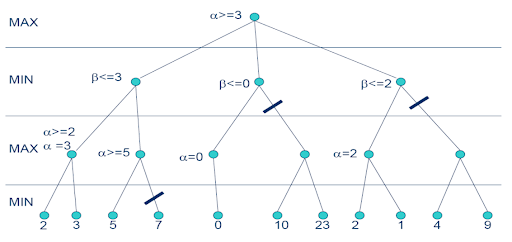
\includegraphics[width=0.8\textwidth]{Figures/Gallery/ab_prun.png}
	\captionof{figure}{Sơ đồ cây tìm kiếm MiniMax có kết hợp cắt tỉa $\alpha$ - $\beta$}
	\label{fig:ab_prun}
\end{center}
Hiệu quả về mặt toán học của phép cắt tỉa Alpha-Beta phụ thuộc hoàn toàn vào thứ tự duyệt các nước đi trên cây trò chơi. Trong trường hợp lý tưởng nhất - khi các nước đi tốt nhất luôn được hệ thống ưu tiên duyệt và đánh giá trước - độ phức tạp thời gian của thuật toán được giảm thiểu một cách đáng kể từ $\mathcal{O}(b^d)$ của Minimax thuần túy xuống chỉ còn:
$$\mathcal{O}\left(b^{\frac{d}{2}}\right)$$

Nói một cách khác, với một thứ tự chọn nước đi hoàn hảo, thuật toán Alpha-Beta có thể giải quyết được một cây trò chơi có độ sâu gấp đôi ($2d$) so với thuật toán Minimax thuần túy trong cùng một quỹ thời gian tính toán. Ngược lại, nếu thứ tự duyệt các nước đi diễn ra hoàn toàn ngẫu nhiên, tổng số nút cần phải kiểm tra đối với một hệ số phân nhánh trung bình sẽ rơi vào khoảng $\mathcal{O}\left(b^{\frac{3d}{4}}\right)$.

Xét về độ phức tạp không gian, do cả hai giải thuật Minimax và Alpha-Beta về bản chất đều vận hành dựa trên nguyên lý duyệt cây theo chiều sâu (DFS), cấu trúc bộ nhớ chỉ đòi hỏi lưu trữ các nút dọc theo một đường đi duy nhất từ nút gốc đến nút lá hiện hành, cùng với các nút anh em chưa được duyệt trực tiếp của chúng. Do đó, độ phức tạp không gian bộ nhớ của thuật toán cắt tỉa vẫn duy trì ổn định ở mức tuyến tính:
$$\mathcal{O}(bd)$$

\section{Giới hạn độ sâu và Hàm đánh giá tĩnh}

Chúng ta không thể xây dựng một cây trò chơi hoàn chỉnh cho trò chơi cờ Caro thay vào đó ta có thể làm như sau:

\begin{itemize}
	\item Giới hạn độ sâu tìm kiếm (tức là xây dựng một cây trò chơi rút gọn đến một độ sâu tối đa nào đó)
	\item Đưa ra một hàm đánh giá heuristic nào đó để đánh giá mức độ tốt hay xấu của mỗi trạng thái nút lá của cây trò chơi đã bị giới hạn độ sâu. 
\end{itemize}

\subsection{Giới hạn độ sâu}

Mặc dù kỹ thuật cắt tỉa $\alpha$ - $\beta$ đã tối ưu hóa mạnh mẽ tiến trình duyệt cây, nhưng đối với những trò chơi có không gian trạng thái khổng lồ như cờ Caro, việc duyệt sâu cho đến khi đạt được trạng thái kết thúc ở tận cuối ván cờ là điều bất khả thi về mặt tài nguyên máy tính. Ở những nước đi đầu tiên, hệ số phân nhánh b có thể lên tới 225, khiến cây trò chơi phình to theo hàm mũ.
Để giải quyết vấn đề bùng nổ tổ hợp này, thuật toán tìm kiếm bắt buộc phải áp dụng kỹ thuật Giới hạn độ sâu. Hệ thống sẽ thiết lập một cơ chế chủ động ngắt tiến trình duyệt cây khi độ sâu tìm kiếm đạt đến một ngưỡng d được định trước (ví dụ trong đồ án này là d=3 hoặc d=4). Tuy nhiên, sự can thiệp này làm nảy sinh một thách thức toán học mới: tại điểm ngắt d, hầu hết các trạng thái bàn cờ đều đang ở cục diện tranh chấp, chưa thực sự kết thúc. Tại các "nút lá tạm thời" này, hệ thống không thể sử dụng hàm Lợi ích đích Utility($s$) để trả về điểm số Thắng/Thua/Hòa tuyệt đối. Nhu cầu cấp thiết lúc này là phải có một cơ chế ước lượng xem cục diện hiện tại đang nghiêng về bên nào, từ đó làm cơ sở để thuật toán Minimax tiếp tục chọn lọc nước đi. 

\subsection{Hàm đánh giá}

Để giải quyết thách thức do việc giới hạn độ sâu để lại, thuật toán sử dụng một Hàm đánh giá (Heuristic Evaluation Function), thường được ký hiệu là $EVAL(s)$, để chấm điểm và ước lượng mức độ lợi thế của cục diện bàn cờ tại trạng thái đó.

Về mặt toán học, hàm $EVAL(s)$ được định nghĩa dưới dạng một hàm tổng tuyến tính có trọng số:
\begin{equation}
	EVAL(s) = w_1 f_1(s) + w_2 f_2(s) + \dots + w_n f_n(s)
\end{equation}

\begin{itemize}
	\item \textbf{$b_i(s)$ (Tần suất xuất hiện):} Đại diện cho số lượng các thế cờ tấn công/phòng thủ cốt lõi (ví dụ: chuỗi 3 quân thoáng hai đầu, chuỗi 4 quân bị chặn) đang tồn tại trên bàn cờ tại trạng thái $s$.
	
	\item \textbf{$w_i$ (Điểm số Heuristic):} Tương ứng với các giá trị điểm số được khai báo tĩnh. Tham số này định lượng mức độ nguy hiểm của từng thế cờ cụ thể (ví dụ: thế 3 thoáng được đánh giá mức độ rủi ro là 670 điểm, trong khi thế 2 thoáng chỉ có 16 điểm).
\end{itemize}

Quá trình tính toán tổng điểm $EVAL(s)$ được hệ thống thực hiện thông qua 3 bước xử lý mảng:
\begin{itemize}
	\item \textbf{Bóc tách tuyến tính:} Hệ thống tiến hành phân rã ma trận bàn cờ $2D$ thành các mảng $1D$ độc lập bao gồm toàn bộ các hàng ngang, cột dọc và các đường chéo. Để tối ưu hóa hiệu năng, thuật toán sẽ chủ động loại bỏ các đường chéo có độ dài nhỏ hơn $4$ ô nhằm tiết kiệm tài nguyên xử lý của CPU, do các cấu trúc ngắn này không đủ không gian hình học để hình thành chuỗi $5$ quân cờ chiến thắng.
	\item \textbf{Quét cửa sổ trượt:} Sử dụng các khung bộ lọc có kích thước linh hoạt (tương ứng từ $4, 5,$ đến $6$ ô cờ) trượt dọc theo từng mảng $1D$ đã bóc tách. Quá trình này giúp hệ thống nhận diện, phân loại mẫu hình và đếm chính xác số lượng tần suất xuất hiện $f_i(s)$ của từng thế cờ chiến thuật đang hiện diện trên bàn cờ.
	\item \textbf{Tính tổng trọng số:} Tiến hành tổng hợp và nhân tích chập ma trận giữa tần suất xuất hiện $f_i(s)$ vừa quét được với bộ điểm số trọng số hằng số $w_i$ được quy định sẵn trong từ điển để trả về giá trị điểm số cuối cùng của hàm tổng $Eval(s)$, làm căn cứ quyết định cho các tầng đệ quy kế tiếp.
\end{itemize}


\section{Hồi quy Logistic}
Hồi quy Logistic là một thuật toán học máy phân lớp thống kê được sử dụng để dự đoán xác suất của một đầu ra nhị phân ($0$ hoặc $1$). Trong bài toán lượng giá trạng thái trò chơi đối kháng, thuật toán này đóng vai trò thiết lập mối quan hệ giữa các đặc trưng cấu trúc trên bàn cờ và khả năng dẫn đến chiến thắng.

Bản chất của Hồi quy Logistic là việc lấy một hàm tổng tuyến tính của các biến đầu vào (đặc trưng thế cờ) và đưa qua một hàm phi tuyến tính gọi là \textbf{hàm Sigmoid} (hoặc hàm Logistic) để ánh xạ kết quả về khoảng giá trị xác suất $(0, 1)$.

Công thức toán học của hàm số Sigmoid có dạng như sau:
\begin{equation}
	\sigma(z) = \frac{1}{1 + e^{-z}}
\end{equation}

Trong đó, biến $z$ đại diện cho một hàm tổ hợp tuyến tính của các đặc trưng đầu vào $x_i$ kết hợp với bộ trọng số hệ số hồi quy $w_i$ tương ứng:
\begin{equation}
	z = w_0 + w_1 x_1 + w_2 x_2 + \dots + w_n x_n
\end{equation}
	
Khi áp dụng vào bài toán, giá trị đầu ra của $\sigma(z)$ đại diện cho xác suất chiến thắng của một trạng thái cục diện bàn cờ hiện hành. Quá trình huấn luyện mô hình thực chất là việc tối ưu hóa hàm mất mát Binary Cross -  Entropy để tìm ra bộ tham số trọng số $w_i$ tối ưu nhất, làm cơ sở khoa học vững chắc cho việc định lượng điểm số Heuristic thay vì thiết lập thủ công.
 
	%----------------------------------------------------------------------------------------
%	CHƯƠNG 3: PHƯƠNG PHÁP NGHIÊN CỨU VÀ THIẾT KẾ HỆ THỐNG
%----------------------------------------------------------------------------------------

\chapter{KIẾN TRÚC VÀ THIẾT KẾ HỆ THỐNG} % Tên của chương
\label{Chapter3}

% =================================================================
%   MỤC 3.1
% =================================================================
\section{Pipeline tổng thể của dự án}
\begin{center}
	\nopagebreak
	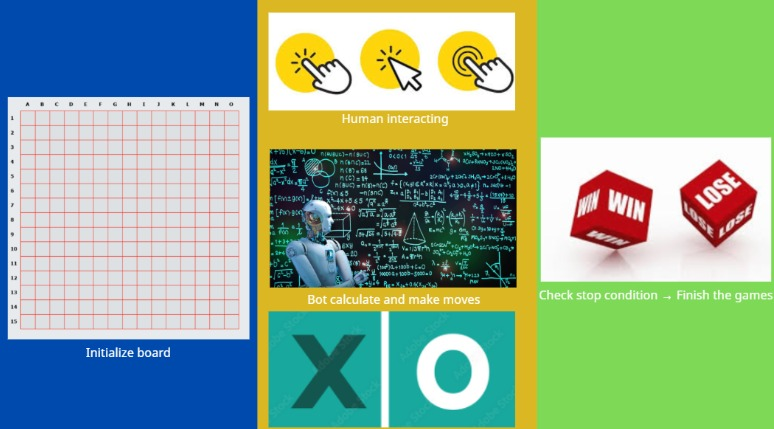
\includegraphics[width=\textwidth]{Figures/Gallery/pipeline.jpg}
	\captionof{figure}{Quy trình xử lý dữ liệu của hệ thống}
	\label{fig:pipeline}
\end{center}
\vspace{0.3cm}
Tiến trình xử lý và truyền dịch trạng thái của trò chơi được chia tách tường minh thành 4 giai đoạn cốt lõi bao gồm:

\begin{itemize}
	\item \textbf{Giai đoạn 1 - Khởi tạo cấu hình và Quản lý trạng thái gốc:} 
	Ngay khi ứng dụng được kích hoạt, hàm khởi tạo thiết lập các tham số kỹ thuật nền tảng bao gồm kích thước ma trận bàn cờ tiêu chuẩn ($10 \times 10$, $12 \times 12$, $15 \times 15$) và độ sâu cây quyết định mặc định cho AI ($\text{depth} = 3$). Hệ thống cấp phát vùng nhớ dọn trống toàn bộ ma trận về giá trị số $0$. Đặc biệt, cơ chế khóa bảo mật đồng bộ \texttt{threading.Lock()} được thiết lập sẵn nhằm chuẩn bị tài nguyên cho các tác vụ tính toán nền song song.
	
	\item \textbf{Giai đoạn 2 - Tương tác người dùng và Ghi nhận lịch sử di chuyển:} 
	Hệ thống lắng nghe các sự kiện phần cứng, đón nhận tọa độ click chuột $(r, c)$ từ người chơi (nhận giá trị toán học là $-1$). Hàm kiểm tra tính hợp lệ sẽ xác minh ô cờ trống trước khi ghi đè dữ liệu lên ma trận \texttt{board[r][c]}. Nước đi hợp lệ ngay lập tức được đóng gói dạng Tuple $(r, c, \text{player})$ đẩy vào ngăn xếp \texttt{move\_history}, đồng thời dịch mã sang định dạng biên bản cờ chuẩn hóa PGN để lưu vào \texttt{pgn\_history} trước khi chuyển đổi trạng thái lượt đi sang đối thủ.
	
	\item \textbf{Giai đoạn 3 - Giới hạn không gian và Tìm kiếm quyết định tối ưu (AI Decision Pipeline):} 
	Khi đến lượt đi của Bot AI (nhận giá trị toán học là $1$), hệ thống kích hoạt một luồng ngầm độc lập (\textit{Worker Thread}) để tránh gây nghẽn giao diện. Luồng phụ thực thi chuỗi tiến trình con:
	\begin{itemize}
		\item \textbf{Bước 1:} Gọi hàm \texttt{get\_interesting\_moves} quét ma trận trong bán kính 1 ô kế cận các quân cờ hiện hành để cô lập vùng tìm kiếm, giảm số lượng nút tiềm năng từ 150 ô xuống tối đa 30 ô để chặn đứng nguy cơ bùng nổ tổ hợp.
		\item \textbf{Bước 2:} Khởi chạy lõi Minimax đệ quy theo chiều sâu (DFS) xuống các tầng trạng thái giả lập.
		\item \textbf{Bước 3:} Xuyên suốt quá trình duyệt, hệ thống liên tục truyền các tham số chặn dưới $\alpha$ và chặn trên $\beta$, thực hiện bẻ gãy vòng lặp duyệt nhánh ngay khi phát hiện điều kiện $\alpha \ge \beta$.
		\item \textbf{Bước 4:} Tại độ sâu giới hạn, hàm \texttt{evaluate\_board\_heuristic} thực hiện cắt chuỗi con đối chiếu với từ điển \texttt{SCORE\_MATRIX} (kết hợp \texttt{ATTACK\_MATRIX} và \texttt{DEFEND\_MATRIX}) để tính toán điểm số tối ưu, trả về tọa độ nước đi tốt nhất tại nút gốc.
	\end{itemize}
	
	\item \textbf{Giai đoạn 4-- Xác định điều kiện dừng ván đấu (Terminal Check):} 
	Sau khi một nước đi được hạ xuống, hàm logic \texttt{check\_win} thực hiện nhiệm vụ quét trạng thái bàn cờ theo 4 hướng địa lý (ngang, dọc, và 2 đường chéo). Thuật toán áp dụng nghiêm ngặt luật chặn hai đầu tiêu chuẩn (\textit{Double-Blocked Rule}), tính toán biến \texttt{blocked\_ends} để đảm bảo chuỗi đạt $\ge 5$ quân cờ và không bị chặn cả 2 đầu thì mới phân định chiến thắng. Khi điều kiện dừng thỏa mãn (thắng-thua hoặc lấp đầy bàn cờ dẫn đến hòa), trạng thái \texttt{game\_over} được gán bằng \texttt{True} để đóng băng tương ứng, đồng thời kích hoạt hàm \texttt{print\_pgn\_final()} xuất toàn bộ biên bản trận đấu ra màn hình điều khiển.
\end{itemize}

\section{Chi tiết kiến trúc phần mềm và cài đặt thuật toán}
\subsection{Thiết kế Module}

Một trong những điểm cải tiến cốt lõi trong kiến trúc phần mềm của đề tài này là việc áp dụng nguyên lý phân tách các thành phần. Thay vì xây dựng một tệp mã nguồn tập trung, hệ thống được chia thành hai module độc lập, giao tiếp với nhau thông qua lập trình hướng đối tượng:
\begin{itemize}
	\item \textbf{Module bộ não xử lý trung tâm (Logic\_game.py):} Đây là thành phần chứa toàn bộ trạng thái dữ liệu của ván cờ. Lớp này chịu trách nhiệm khởi tạo ma trận bàn cờ, ghi nhận lịch sử nước đi, kiểm tra điều kiện chiến thắng và thực thi các giải thuật Minimax, Heuristic. Điểm đặc biệt là lớp CaroLogic hoàn toàn độc lập với môi trường đồ họa, không chứa bất kỳ mã nguồn nào liên quan đến thư viện hiển thị Pygame, giúp nó có tính tái sử dụng cao.
	\item \textbf{Module giao diện đồ họa (UI.py):} Thành phần này đóng vai trò là giao diện tương tác trực tiếp với người sử dụng. Nó chịu trách nhiệm khởi tạo cửa sổ ứng dụng bằng thư viện Pygame, hiển thị hình ảnh màu sắc hệ Dark Mode, quản lý hệ thống âm thanh hiệu ứng (SFX) và lắng nghe các sự kiện phần cứng như click chuột hoặc nhập liệu văn bản.
\end{itemize}

\subsection{Quản lý trạng thái và tính năng bổ trợ (State Management)}
Trạng thái của một ván cờ được lớp \texttt{CaroLogic} quản lý động thông qua hệ thống lưu vết lịch sử di chuyển, cho phép triển khai các tính năng bổ trợ nâng cao nhằm tối ưu hóa trải nghiệm người dùng:
\begin{itemize}
	\item \textbf{Cơ chế hoạt động của tính năng Undo (Đi lại):} Tính năng này được cài đặt dựa trên cấu trúc dữ liệu Ngăn xếp (\textit{Stack}) tuyến tính. Toàn bộ các nước đi của người chơi và Bot AI sau khi thực hiện thành công sẽ được đóng gói dưới dạng Tuple $(r, c, \text{player})$ và đẩy vào mảng \texttt{move\_history}. Đồng thời, ký hiệu định dạng biên bản PGN cũng được lưu vào \texttt{pgn\_history}. Khi người chơi kích hoạt lệnh Undo (thông qua phím tắt U trên bàn phím hoặc click nút UNDO trên Control Panel), hàm \texttt{undo\_move} sẽ thực hiện lệnh giải phóng bộ nhớ bằng cách rút (\texttt{.pop()}) liên tiếp hai phần tử cuối cùng ra khỏi ngăn xếp lịch sử (tương ứng với một nước cờ của máy và một nước cờ của người). Hệ thống tiến hành đặt lại giá trị ma trận tại hai vị trí đó về bằng $0$ (ô trống), xóa biên bản tương ứng và trả lại lượt đi cho con người.
	\item \textbf{Cơ chế hoạt động của tính năng Reset (Làm mới) và Menu Trận đấu:} Tính năng Reset (phím tắt R hoặc nút RESET) kích hoạt hàm \texttt{reset\_game} giúp xóa trắng toàn bộ ma trận bàn cờ về $0$ và dọn rác các mảng lịch sử mà không cần phải khởi động lại toàn bộ chương trình. Trong khi đó, vòng lặp \texttt{show\_menu} cung cấp một giao diện cấu hình trực quan trước trận đấu. Người dùng có thể tác động lên các nút bấm để thay đổi trực tiếp các tham số cấu hình của lớp \texttt{CaroLogic} bao gồm kích thước ma trận (\texttt{board\_size} nhận các giá trị $10, 12, 15$) và độ sâu cây tìm kiếm quyết định (\texttt{bot\_depth} nhận các giá trị $1, 2, 3$).
\end{itemize}

\subsection{Tối ưu hóa hiệu năng bằng Đa luồng (Multi-threading)}
Đối với các ứng dụng giao diện đồ họa (GUI), việc duy trì tốc độ phản hồi mượt mà của khung hình là yếu tố tiên quyết. Tuy nhiên, thuật toán tìm kiếm Minimax ở độ sâu lớn ($\text{Depth} = 3$) đòi hỏi một khối lượng tính toán khổng lồ và tốn từ 1 đến vài giây để đưa ra kết quả. Nếu tiến trình này được thực thi trực tiếp trên luồng chạy chính (\textit{Main Thread} - nơi đảm nhận nhiệm vụ vẽ giao diện và bắt sự kiện Pygame), hệ điều hành sẽ rơi vào trạng thái tắc nghẽn, gây ra hiện tượng treo cửa sổ.

Để giải quyết triệt để bài toán hiệu năng này, hệ thống áp dụng kỹ thuật Lập trình đa luồng (\textit{Multi-threading}) thông qua thư viện \texttt{threading} tích hợp sẵn của Python:
\begin{itemize}
	\item \textbf{Phân chia luồng xử lý (Threading Workers):} Luồng chính (\textit{Main Thread}) được giải phóng hoàn toàn khỏi các tác vụ tính toán nặng, chỉ tập trung duy nhất vào vòng lặp vẽ màn hình \texttt{draw\_ui} cố định ở tốc độ $30$ khung hình/giây ($30$ FPS). Khi đến lượt của Bot AI di chuyển hoặc khi người chơi nhấn nút yêu cầu trợ giúp nước đi, lớp \texttt{CaroUI} sẽ lập tức khởi tạo một luồng ngầm độc lập (\textit{Worker Thread}) thông qua lệnh \texttt{threading.Thread(target=..., daemon=True).start()} tương ứng cho các hàm \texttt{bot\_calculation\_worker} hoặc \texttt{hint\_calculation\_worker}. Tiến trình tính toán Minimax sẽ chạy song song ở chế độ nền. Khi tìm ra nước đi tối ưu, luồng phụ này sẽ cập nhật kết quả vào bộ nhớ chung và tự động kết thúc ván đóng luồng.
	\item \textbf{Cơ chế Khóa bảo mật đồng bộ (\texttt{threading.Lock}):} Do hệ thống vận hành theo mô hình đa luồng truy cập đồng thời vào một vùng tài nguyên chung (Ma trận dữ liệu \texttt{self.logic.board}), nguy cơ xảy ra lỗi tranh chấp dữ liệu (\textit{Race Condition}) là cực kỳ cao. Ví dụ: luồng chính đang đọc ma trận để vẽ quân cờ lên màn hình trong khi luồng phụ AI đang ghi đè thay đổi giá trị để giả lập nước đi Minimax. Để ngăn chặn xung đột, nhóm sử dụng cơ chế khóa đồng bộ độc quyền thông qua đối tượng \texttt{self.lock = threading.Lock()} trong lớp \texttt{CaroLogic}. Bằng cú pháp \texttt{with self.logic.lock:} (hoặc \texttt{with self.lock:}), luồng đang thực thi sẽ chiếm quyền kiểm soát két sắt dữ liệu, ép tất cả các luồng khác phải rơi vào trạng thái chờ (\textit{Block}) cho đến khi luồng hiện tại xử lý xong dòng code và mở khóa. Cơ chế này đảm bảo tính toàn vẹn dữ liệu tuyệt đối cho hệ thống trò chơi.
\end{itemize}

\subsection{Cài đặt thuật toán hệ thống}

\subsubsection{Thiết lập trọng số Hàm đánh giá}
Trọng tâm sức mạnh tư duy của Bot AI nằm ở việc thiết lập các giá trị hằng số trong bộ từ điển điểm số \texttt{SCORE\_MATRIX}. Để tạo ra một đối thủ có lối chơi thực tế, thông minh và biết tùy biến theo thế trận, nhóm đã áp dụng chiến lược lai giữa cấu trúc mẫu hình hình học (\textit{Pattern Matching}) và tư duy công -- thủ biệt lập:
\begin{itemize}
	\item \textbf{Chiến lược ma trận tấn công (\texttt{ATTACK\_MATRIX}):} Định nghĩa giá trị điểm số dương cho các chuỗi quân cờ của riêng AI (mang giá trị $1$ trên ma trận). Điểm số được phân cấp nhảy vọt để ưu tiên tuyệt đối cho các nước đi dứt điểm ván đấu: chuỗi 5 quân thắng chắc nhận $200.000$ điểm, thế cờ 4 quân mở 2 đầu nhận $11.000$ điểm, và giảm dần về các thế cờ tạo chuỗi 3 hoặc chuỗi 2.
	\item \textbf{Chiến lược ma trận phòng thủ (\texttt{DEFEND\_MATRIX}):} Định nghĩa giá trị điểm phạt (mang dấu âm) cho các cấu hình quân cờ của người chơi (mang giá trị $-1$ trên ma trận). 
	\item \textbf{Nguyên lý ép phòng thủ:} Điểm nhấn kỹ thuật đặc biệt ở đây là trị tuyệt đối của điểm phòng thủ luôn cao hơn điểm tấn công tại các ngưỡng thế cờ nguy cấp. Cụ thể, khi người chơi đạt thế 4 quân mở hai đầu, AI sẽ gán điểm phạt cực nặng là $-45.000$ điểm. Khi so sánh với điểm thưởng của thế tấn công 4 quân mở hai đầu của riêng mình ($11.000$ điểm), thuật toán Minimax buộc phải lựa chọn nước đi chặn đứng chuỗi cờ của đối thủ. Chiến lược này giúp AI ngăn chặn tối đa việc bị mắc bẫy ở các nước đi xa.
\end{itemize}

Sau khi định nghĩa, hai ma trận được gộp lại làm một thông qua cú pháp giải nén từ điển \texttt{SCORE\_MATRIX = \{**ATTACK\_MATRIX, **DEFEND\_MATRIX\}} của ngôn ngữ Python để thuật toán tìm kiếm tối ưu hóa tốc độ tra cứu cấu trúc dữ liệu với độ phức tạp $\mathcal{O}(1)$.

\begin{table}[!htbp]
	\centering
	\renewcommand{\arraystretch}{1.25}
	\caption{Bảng trọng số lượng giá trong cấu hình hàm đánh giá Heuristic}
	\label{tab:score_matrix}
	\begin{tabular}{|c|c|c|c|}
		\hline
		\textbf{Thế cờ (Pattern)} & \textbf{Trạng thái mô tả} & \textbf{Điểm Tấn công} & \textbf{Điểm Phòng thủ} \\ \hline
		\texttt{X X X X X} & 5 quân liên tiếp (Thắng) & $+200.000$ & $-200.000$ \\ \hline
		\texttt{- X X X X -} & 4 quân mở 2 đầu & $+11.000$ & $-45.000$ \\ \hline
		\texttt{O X X X X -} & 4 quân bị chặn 1 đầu & $+2.700$ & $-2.700$ \\ \hline
		\texttt{- X X X -} & 3 quân mở 2 đầu & $+670$ & $-1.500$ \\ \hline
		\texttt{- X X - X -} & 3 quân đứt đoạn & $+500$ & $-1.000$ \\ \hline
		\texttt{O X X X -} & 3 quân mở 1 đầu / Bị chặn & $+210$ & $-210$ \\ \hline
		\texttt{- X X -} & 2 quân mở 2 đầu & $+16$ & $-16$ \\ \hline
	\end{tabular}
\end{table}

\subsubsection{Cơ chế phân cấp 3 mức độ khó (\texttt{BOT\_DEPTH})}
Để trò chơi tiếp cận được nhiều đối tượng người dùng, lớp \texttt{CaroLogic} cài đặt biến cấu hình \texttt{bot\_depth} nhận 3 giá trị tương ứng với 3 cấp độ thông minh độc lập của Bot AI:
\begin{itemize}
	\item \textbf{Cấp độ Dễ (\texttt{bot\_depth} = 1):} Tại cấp độ này, thuật toán Minimax chỉ tìm kiếm ở độ sâu duy nhất là 1 bước đi kế tiếp. Đồng thời, tại hàm lọc nước đi, AI bị giới hạn nghiêm ngặt chỉ lấy 5 nước đi ngẫu nhiên đầu tiên xuất hiện trên bảng. Kết quả là AI chỉ có khả năng nhìn thấy các cơ hội ăn điểm trực tiếp hoặc nguy cơ thua ngay lập tức ở lượt sau, tạo nên một lối đánh ngây ngô, dễ mắc bẫy, phù hợp cho người chơi mới.
	\item \textbf{Cấp độ Trung bình (\texttt{bot\_depth} = 2):} Cây quyết định duyệt sâu xuống 2 tầng trạng thái (AI giả định nước đi của mình và một nước đáp trả tiếp theo của con người). Hàm lọc được nới rộng, tiến hành sắp xếp các nước đi tiềm năng theo bán kính tính từ tâm bàn cờ ra ngoài và cắt lấy tối đa 30 nước đi có điểm Heuristic cao nhất để đưa vào Minimax. Bot AI ở cấp độ này thời gian phản hồi rất nhanh, có khả năng phòng thủ và tấn công tương đối tốt nhưng thi thoảng vẫn bị lọt bẫy nếu người chơi kéo giãn quân cờ ra các vùng biên của bàn cờ.
	\item \textbf{Cấp độ Khó (\texttt{bot\_depth} = 3):} Thuật toán duyệt sâu xuống 3 tầng trạng thái đầy đủ trên cây quyết định. Ở cấp độ này, tham số giới hạn số lượng nước đi bị loại bỏ hoàn toàn, ép AI phải vét cạn tất cả các ô trống có khả năng phát sinh điểm. Kết hợp với việc cộng trừ tham số \texttt{depth} trực tiếp vào điểm số trả về ($1.000.000 + \text{depth}$ khi thắng hoặc $-1.000.000 - \text{depth}$ khi thua), AI được tối ưu hóa tư duy để luôn tìm cách chiến thắng với số nước đi ngắn nhất hoặc kéo dài sự sống lâu nhất có thể khi rơi vào thế thua.
\end{itemize}

\subsubsection{Thuật toán thu hẹp vùng tìm kiếm (\texttt{get\_interesting\_moves})}
Đối với một bàn cờ kích thước lớn như $15 \times 15$, tổng số ô trống ở giai đoạn giữa trận đấu có thể lên đến hơn $150$ ô. Nếu tung toàn bộ các ô trống này vào hàm đệ quy Minimax với $\text{Depth} = 3$, số lượng nút lá phát sinh trên cây quyết định sẽ tăng theo cấp số nhân ($150^3 = 3.375.000$ trạng thái), gây sập nguồn tài nguyên xử lý của CPU.

Để tối ưu hóa, nhóm đã cài đặt thuật toán lọc phân vùng thông minh thông qua hàm \texttt{get\_interesting\_moves}:
\begin{enumerate}
	\item Hàm tiến hành duyệt qua toàn bộ ma trận bàn cờ hiện tại.
	\item Tại các vị trí ô cờ đã được đánh quân, hàm sẽ quét rộng ra xung quanh theo 8 hướng hình học với bán kính rộng 1 ô cờ.
	\item Nếu phát hiện ô xung quanh là ô trống, tọa độ của ô đó sẽ được thêm vào cấu trúc dữ liệu \texttt{set()} (Tập hợp) nhằm tự động loại bỏ các tọa độ trùng lặp.
	\item Cuối cùng, tập hợp được chuyển đổi ngược về dạng mảng tuyến tính \texttt{move\_list}.
\end{enumerate}
Việc thu hẹp vùng tìm kiếm xuống bán kính 1 ô giúp AI cô lập hoàn toàn các ô trống vô ích ở vùng biên xa, giảm số lượng nước đi tiềm năng đưa vào Minimax từ $150$ ô xuống chỉ còn từ $15$ đến $35$ ô tùy giai đoạn trận đấu. Kỹ thuật này giúp giảm tải hơn $80\%$ khối lượng duyệt cây, đảm bảo thời gian tính toán nước đi chế độ Khó luôn duy trì ổn định.

\subsection{Ứng dụng mô hình Hồi quy Logistic trong tối ưu hóa bộ trọng số lượng giá}

Để loại bỏ tính cảm tính và tối ưu hóa các giá trị điểm số trong từ điển \texttt{SCORE\_MATRIX}, hệ thống triển khai mô hình học máy Hồi quy Logistic nhằm tự động hóa tiến trình khai phá dữ liệu và gán trọng số cho các mẫu hình chiến thuật. Quy trình hiện thực hóa giải pháp này được cấu trúc qua các giai đoạn tính toán chi tiết sau:

\subsubsection{Thu thập dữ liệu và biểu diễn không gian vectơ đặc trưng}
Dữ liệu huấn luyện được tổng hợp từ tập mẫu gồm các biên bản trận đấu chất lượng cao. Tại mỗi trạng thái bàn cờ $s$, cục diện được trích xuất và ánh xạ thành một vectơ đặc trưng $X = [x_1, x_2, \dots, x_n]^T$, trong đó mỗi phần tử $x_i$ đại diện cho tần suất xuất hiện $f_i(s)$ của mẫu hình thứ $i$ (ví dụ: số lượng thế cờ $4$ quân mở hai đầu, $3$ quân bị chặn một đầu).

Mỗi vectơ đặc trưng $X$ đi kèm với một nhãn mục tiêu nhị phân $y \in \{0, 1\}$ được xác định dựa trên kết quả cuối cùng của ván đấu:
\begin{equation}
	y = \begin{cases} 
		1 & \text{nếu trạng thái } s \text{ dẫn đến chiến thắng chung cuộc cho AI} \\
		0 & \text{nếu trạng thái } s \text{ dẫn đến thất bại hoặc hòa}
	\end{cases}
\end{equation}

\subsubsection{Cơ chế ước lượng xác suất bằng hàm kích hoạt phi tuyến}
Mô hình tiến hành thiết lập một hàm tổ hợp tuyến tính giữa vectơ đặc trưng $X$ và bộ trọng số hệ số hồi quy tương ứng $W = [w_1, w_2, \dots, w_n]^T$, kết hợp với sai số ngẫu nhiên $w_0$:
\begin{equation}
	z = w_0 + \sum_{i=1}^{n} w_i x_i
\end{equation}

Để chuyển đổi giá trị lượng giá $z$ từ không gian số thực vô hạn $(-\infty, +\infty)$ về không gian xác suất giới hạn $(0, 1)$, hệ thống đưa $z$ qua hàm kích hoạt Sigmoid toán học:
\begin{equation}
	P(y=1|X) = \hat{y} = \sigma(z) = \frac{1}{1 + e^{-z}}
\end{equation}
Trong đó, giá trị $\hat{y}$ phản ánh một cách chính xác tỷ lệ phần trăm cơ hội giành chiến thắng của tác tử AI khi sở hữu tổ hợp thế cờ hiện tại.

\subsubsection{Tối ưu hóa hàm mất mát và trích xuất điểm số Heuristic}
Quá trình huấn luyện mô hình thực chất là việc tìm kiếm bộ tham số $W$ sao cho khoảng cách giữa xác suất dự đoán $\hat{y}$ và nhãn thực tế $y$ là nhỏ nhất. Hệ thống áp dụng hàm mất mát Entropy chéo nhị phân (\textit{Binary Cross-Entropy Loss}) trên toàn bộ tập dữ liệu gồm $M$ mẫu:
\begin{equation}
	J(W) = -\frac{1}{M} \sum_{j=1}^{M} \left[ y^{(j)} \log(\hat{y}^{(j)}) + (1 - y^{(j)}) \log(1 - \hat{y}^{(j)}) \right]
\end{equation}

Thuật toán tối ưu hóa hạ gradient (\textit{Gradient Descent}) được kích hoạt để liên tục cập nhật trọng số theo chiều ngược pha với đạo hàm riêng:
\begin{equation}
	w_i \leftarrow w_i - \alpha \frac{\partial J(W)}{\partial w_i}
\end{equation}

Sau khi mô hình đạt trạng thái hội tụ, các hệ số hồi quy $w_i$ trích xuất được phản ánh trực tiếp mức độ đóng góp khoa học và tỷ lệ ảnh hưởng của từng mẫu hình đến khả năng chiến thắng cục diện. Khác với việc gán tay cảm tính, các hệ số thực nghiệm này tồn tại dưới dạng số thập phân có độ mịn cao. Hệ thống tiến hành chuẩn hóa và nạp trực tiếp các giá trị này vào hai ma trận \texttt{ATTACK\_MATRIX\_LOGISTIC} và \texttt{DEFEND\_MATRIX\_LOGISTIC} phục vụ cho lõi tìm kiếm Minimax, chi tiết thông số được thể hiện tại Bảng \ref{tab:weights_logistic}.

\begin{table}[!htbp]
	\centering
	\renewcommand{\arraystretch}{1.25}
	\caption{Hệ thống trọng số thực nghiệm tối ưu bằng Hồi quy Logistic}
	\label{tab:weights_logistic}
	\begin{tabular}{|c|c|c|c|}
		\hline
		\textbf{Thế cờ (Pattern)} & \textbf{Trạng thái mô tả} & \textbf{Điểm Tấn công} & \textbf{Điểm Phòng thủ} \\ \hline
		\texttt{X X X X X} & 5 quân liên tiếp (Thắng) & $+200.000,00$ & $-200.000,00$ \\ \hline
		\texttt{- X X X X -} & 4 quân mở 2 đầu & $+14.780,71$ & $-200.000,00$ \\ \hline
		\texttt{O X X X X -} & 4 quân bị chặn 1 đầu & $+18.888,35$ & $-23.248,95$ \\ \hline
		\texttt{- X X - X -} & 3 quân đứt đoạn & $+14.685,24$ & $-17.230,00$ \\ \hline
		\texttt{- X X X -} & 3 quân mở 2 đầu & $+2.908,00$ & $-3.550,76$ \\ \hline
		\texttt{O X X X -} & 3 quân mở 1 đầu & $+4.031,00$ & $-8.598,42$ \\ \hline
		\texttt{- X X -} & 2 quân mở 2 đầu & $+3.736,00$ & $-2.389,63$ \\ \hline
	\end{tabular}
\end{table}
Từ kết quả trên, ta có thể thấy thuật toán học máy đã tinh chỉnh bộ điểm số lệch hẳn so với việc gán tay cảm tính. Ví dụ, trạng thái phòng thủ chống lại chuỗi 4 quân mở 2 đầu (\texttt{- X X X X -}) được thuật toán đẩy giá trị tuyệt đối lên mức tối đa ($-200.000,00$), ngang bằng với việc đối phương có 5 quân liên tiếp. Điều này cho thấy mô hình đã tự học được quy luật: khi đối phương đạt thế trận 4 quân mở 2 đầu thì tỉ lệ thua trận là tuyệt đối, từ đó ép tác tử AI phải ưu tiên chặn đứng thế cờ này bằng mọi giá. Các giá trị thập phân chi tiết giúp hàm lượng giá tĩnh phân tách rạch ròi độ ưu tiên của các nút trên cây tìm kiếm Minimax, giúp Bot đưa ra các quyết định thực tế và tối ưu hơn.
	%----------------------------------------------------------------------------------------
%	CHƯƠNG 4: KẾT QUẢ THỰC NGHIỆM VÀ NHẬN XÉT
%----------------------------------------------------------------------------------------

\chapter{KẾT QUẢ THỰC NGHIỆM VÀ NHẬN XÉT}
\label{Chapter4}

% =================================================================
%   MỤC 4.1
% =================================================================
\section{Kết quả thiết kế giao diện}
\begin{center}
	\nopagebreak
	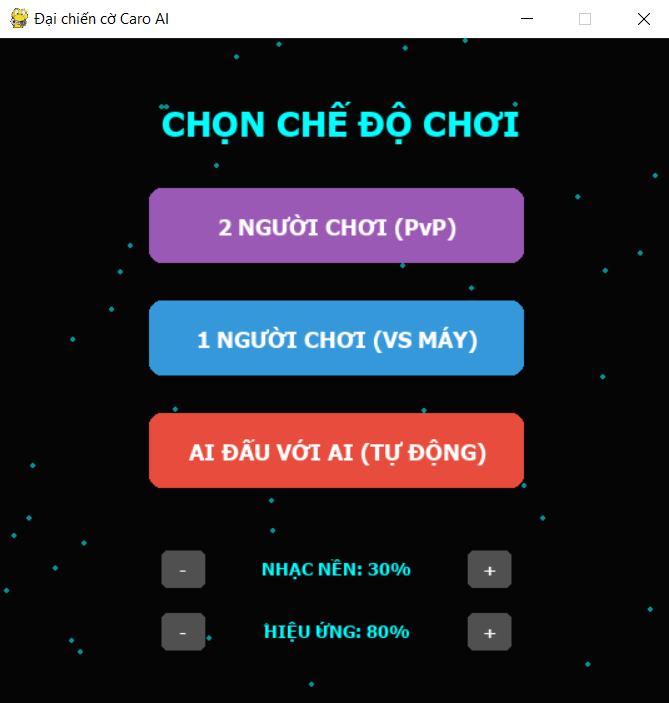
\includegraphics[width=\textwidth]{Figures/Gallery/mode.png}
	\captionof{figure}{Màn hình Menu cấu hình chế độ chơi}
	\label{fig:mode_choosin}
\end{center}
\vspace{0.3cm}
\textbf{Màn hình Chọn chế độ chơi:} Giao diện sử dụng hiệu ứng các hạt trôi nổi tạo chiều sâu không gian. Hệ thống cung cấp 3 chế độ chơi: 2 Người chơi (PvP), 1 Người chơi với máy (PvE), cho AI tự đấu (EvE).
\begin{center}
	\nopagebreak
	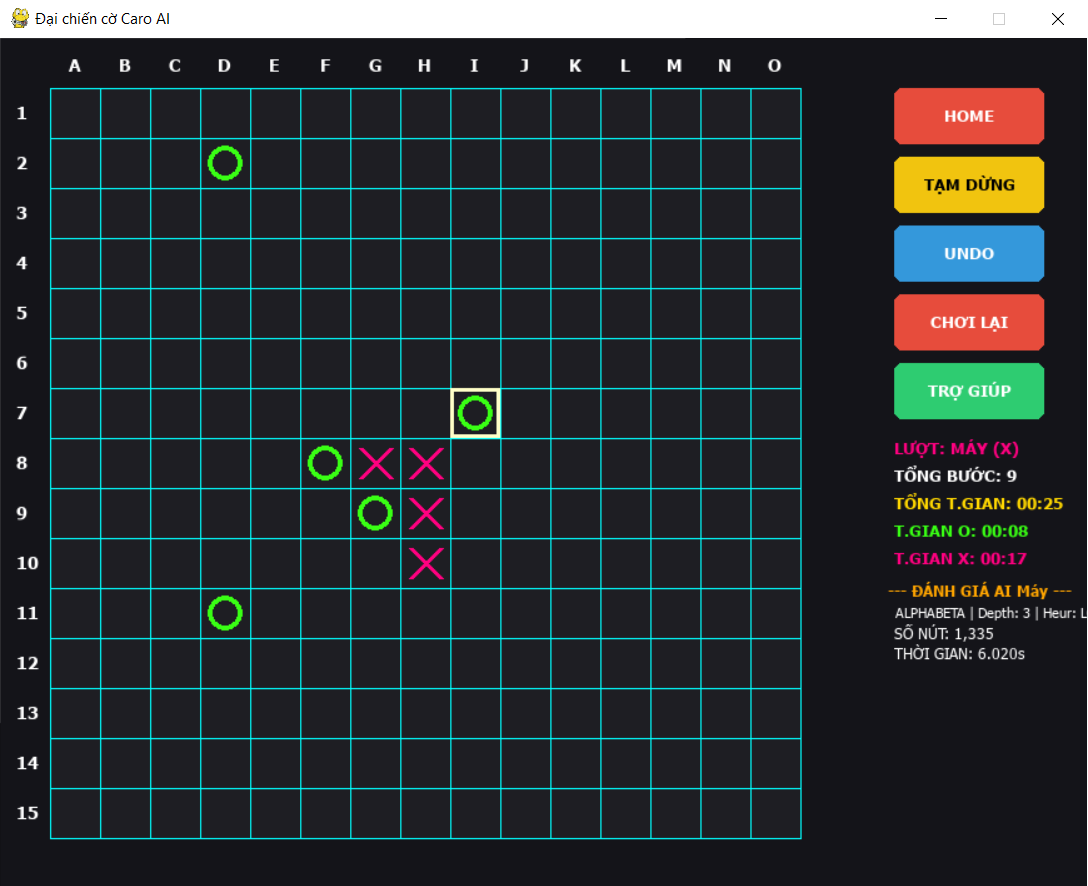
\includegraphics[width=\textwidth]{Figures/Gallery/play.png}
	\captionof{figure}{Giao diện trò chơi}
	\label{fig:gameplay}
\end{center}
\vspace{0.3cm}
\textbf{Đồ họa Neon:} Bàn cờ sử dụng lưới. Quân X (Hồng) và O (Xanh lá) nhằm tăng độ tương phản và chống mỏi mắt.

\textbf{Hệ thống Phản hồi trực quan:}
\begin{itemize}
	\item Tự động đánh dấu viền vàng cho nước đi mới nhất.
	\item Hiển thị viền cam nét đứt tại vị trí AI gợi ý đánh.
	\item Tạo hiệu ứng chớp nháy viền vàng làm nổi bật chuỗi 5 quân cờ chiến thắng.
\end{itemize}
\textbf{Xử lý trạng thái kết thúc:} Tự động ngắt nhạc nền, phát SFX Thắng/Thua. Quá trình giải phóng bộ nhớ và chuyển về Menu được kích hoạt mượt mà chỉ bằng một thao tác click chuột.
	
\begin{center}
	\nopagebreak
	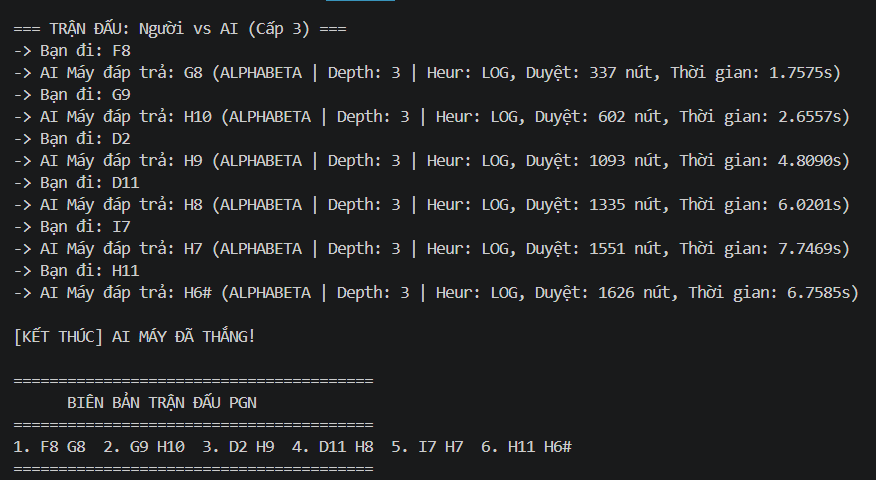
\includegraphics[width=\textwidth]{Figures/Gallery/result.png}
	\captionof{figure}{Màn hình Menu cấu hình chế độ chơi}
	\label{fig:result}
\end{center}
\vspace{0.3cm}
Hệ thống ghi nhận diễn biến trận đấu trên Terminal thông qua hai cơ chế:
\begin{itemize}
	\item In tọa độ từng nước đi theo thời gian thực (nước quyết định được đánh dấu).
	\item Xuất PGN: Tự động tổng hợp mảng lịch sử thành văn bản chuẩn PGN quốc tế ngay khi ván cờ kết thúc để phục vụ lưu trữ và phân tích.
\end{itemize}

\section{Các chỉ số đánh giá hiệu năng và năng lực của tác tử AI}

Để đánh giá một cách toàn diện hiệu quả của các kỹ thuật tối ưu hóa được đề xuất, nhóm thực hiện đề tài tiến hành nghiệm thu và khảo sát năng lực vận hành của hệ thống dựa trên cả hai phương diện: chỉ số hiệu năng tính toán định lượng và năng lực chiến thuật định tính.

\subsection{Khảo sát chỉ số hiệu năng tính toán thực tế (Định lượng)}
Nhóm chỉ số này đo lường mức độ tối ưu phần cứng và tốc độ xử lý của thuật toán tại các độ sâu tìm kiếm $d$ khác nhau thông qua môi trường đối kháng trực tiếp giữa Người và Máy (Human vs AI). 

Các tiêu chí định lượng bao gồm thời gian phản hồi trung bình cho một nước đi, tổng số nút trạng thái ma trận bàn cờ giả định mà CPU phải khởi tạo, duyệt thực tế và điểm số lượng giá tương ứng được chi tiết hóa tại Bảng \ref{tab:hieunang_thuc_te}.

\begin{table}[!htbp]
	\centering
	\renewcommand{\arraystretch}{1.3}
	\caption{Hiệu suất vận hành thực tế của giải thuật tích hợp theo từng cấp độ sâu}
	\label{tab:hieunang_thuc_te}
	\begin{tabular}{|c|c|c|l|}
		\hline
		\textbf{Cấp độ thiết lập} & \textbf{Thời gian phản hồi} & \textbf{Số nút duyệt thực tế} & \textbf{Năng lực tư duy (Định tính)} \\ \hline
		\textbf{Dễ ($d=1$)} & $\sim 0,008$ s & $5 \to 10$ nút & Sơ cấp\\ \hline
		\textbf{Vừa ($d=2$)} & $0,15 \to 0,8$ s & $100 \to 500$ nút & Trung bình\\ \hline
		\textbf{Khó ($d=3$)} & $0,15 \to 4,0$ s & $350 \to 3.500$ nút & Khá \\ \hline
		\textbf{Siêu khó ($d=4$)} & $\ge 3,0$ s & $\ge 2.500$ nút  & Cao cấp \\ \hline
	\end{tabular}
\end{table}

\paragraph{Nhận xét hệ số kiểm thử hiệu suất định lượng:}
\begin{itemize}
	\item \textbf{Sự bùng nổ tổ hợp trạng thái theo chiều sâu:} Đúng như quy luật toán học của cấu trúc cây quyết định, khi độ sâu tăng từ $d=1$ lên $d=4$, cả số lượng nút duyệt lẫn thời gian phản hồi đều tăng trưởng rõ rệt theo hàm mũ $\mathcal{O}(b^d)$ (với $b$ là hệ số nhánh cờ). Tại cấp độ Siêu khó ($d=4$), do không gian trạng thái giả lập quá lớn, thời gian tính toán có xu hướng kéo dài vượt ngưỡng $3,0$ giây ở giai đoạn trung cuộc. Điều này minh chứng cho tính đúng đắn của việc lựa chọn cấu hình mặc định $d=3$ ở giao diện hệ thống nhằm cân bằng tối ưu giữa năng lực tư duy thông minh và trải nghiệm thời gian thực của người dùng.
	\item \textbf{Hiệu quả của giải thuật thu hẹp vùng tìm kiếm:} Nhờ việc áp dụng hàm lọc nước đi tiềm năng \texttt{get\_interesting\_moves} để cô lập bán kính quét xung quanh các quân cờ hiện hành, số lượng nút duyệt ở cấp độ Khó ($d=3$) đã được kìm hãm thành công trong khoảng tuyến tính từ $350$ đến $3.500$ nút thay vì hàng triệu nút trên lý thuyết bàn cờ $15 \times 15$ vắng dòng lọc. Yếu tố này giúp thời gian phản hồi giữ vững ở mức tối ưu, hoàn toàn đáp ứng tiêu chuẩn mượt mà của một ứng dụng trò chơi tương tác.
\end{itemize}

\subsection{Khảo sát năng lực chiến thuật qua đối chiến giả lập (Định tính)}
Để đánh giá định tính năng lực xử lý chiến thuật và chứng minh sự tương quan trực tiếp giữa cấu hình thuật toán và kết quả thắng bại một cách tuyệt đối, hệ thống kích hoạt môi trường giả lập cho hai thực thể Bot tự đối đầu độc lập (AI vs AI) dưới hai kịch bản phân tách.

\textbf{Kịch bản 1: Khảo sát sự ảnh hưởng của chiều sâu cây quyết định ($d$)}

Thực nghiệm tiến hành cho hai tác tử sở hữu cùng thuật toán cải tiến hoàn chỉnh nhưng bất đối xứng về độ sâu tìm kiếm nhằm kiểm thử tính áp đảo hình học. Kết quả các cặp đấu đối kháng được thống kê tại Bảng \ref{tab:ai_vs_ai_depth}.

\begin{table}[!htbp]
	\centering
	\renewcommand{\arraystretch}{1.25}
	\caption{Ma trận kết quả đối đầu giữa các cấp độ sâu trên cùng giải thuật tích hợp}
	\label{tab:ai_vs_ai_depth}
	\begin{tabular}{|c|c|c|c|c|}
		\hline
		\textbf{Quân X $\backslash$ Quân O} & \textbf{$d = 1$} & \textbf{$d = 2$} & \textbf{$d = 3$} & \textbf{$d = 4$} \\ \hline
		\textbf{$d = 1$} & Quân O thắng & Quân O thắng & Quân O thắng & Quân O thắng \\ \hline
		\textbf{$d = 2$} & Quân X thắng & Quân O thắng & Quân O thắng & Quân O thắng \\ \hline
		\textbf{$d = 3$} & Quân X thắng & Quân X thắng & Quân O thắng & Quân O thắng \\ \hline
		\textbf{$d = 4$} & Quân X thắng & Quân X thắng & Quân X thắng & Quân O thắng \\ \hline
	\end{tabular}
\end{table}

\textbf{Kịch bản 2: Khảo sát năng lực xử lý giữa các tổ hợp biến thể giải thuật}

Thực nghiệm tiến hành cấu hình cố định độ sâu ở mức $d=2$ để tập trung kiểm thử tốc độ và khả năng dứt điểm trận đấu giữa các tầng kiến trúc logic cốt lõi bao gồm Minimax thuần túy, Minimax tích hợp Heuristic, và Minimax cải tiến hoàn chỉnh. Kết quả chi tiết tiến trình đối kháng được ghi nhận tại Bảng \ref{tab:ai_vs_ai_variants}.

\begin{table}[!htbp]
	\centering
	\renewcommand{\arraystretch}{1.25}
	\small
	\caption{Ma trận đối chiến và thời gian xử lý thực tế giữa các tổ hợp biến thể giải thuật ($d=2$)}
	\label{tab:ai_vs_ai_variants}
	\begin{tabular}{|m{3.5cm}|m{3.0cm}|m{3.3cm}|m{4.2cm}|}
		\hline
		\textbf{Quân X $\backslash$ Quân O} & \textbf{Minimax thuần túy} & \textbf{Minimax + Heuristic} & \textbf{Minimax + Alpha-Beta + Heuristic} \\ \hline
		\textbf{Minimax thuần túy} & X thắng \newline ($t: 0.001\text{s} \to 0.5\text{s}$ cả X, O) & O thắng \newline ($t: 0.001\text{s} \to 0.5\text{s}$ quân X \newline $0.09\text{s} \to 0.64\text{s}$ quân O) & O thắng \newline ($t: 0.001\text{s} \to 0.5\text{s}$ quân X \newline $0.01\text{s} \to 0.56\text{s}$ quân O) \\ \hline
		\textbf{Minimax + Heuristic} & X thắng \newline ($t: 0.001\text{s} \to 0.5\text{s}$ quân O \newline $0.13\text{s} \to 0.77\text{s}$ quân O) & O thắng \newline ($t: 1\text{s} \to 7\text{s}$ cả X, O) & O thắng \newline ($t: 0.14\text{s} \to 2.8\text{s}$ quân X \newline $0.15\text{s} \to 0.4\text{s}$ quân O) \\ \hline
		\textbf{Minimax + Alpha-Beta + Heuristic} & X thắng \newline ($t: 0.001\text{s} \to 0.5\text{s}$ quân X \newline $0.06\text{s} \to 0.52\text{s}$ quân O) & O thắng \newline ($t: 1\text{s} \to 7\text{s}$ quân O \newline $0.15\text{s} \to 0.4\text{s}$ quân X) & O thắng \newline ($t: 0.15\text{s} \to 1.8\text{s}$ cả X, O) \\ \hline
	\end{tabular}
\end{table}

\paragraph{Nhận xét chuyên sâu từ kết quả đối chiến giả lập:}
\begin{itemize}
	\item \textbf{Sự áp đảo của chiều sâu duyệt cây (Depth):} Minh chứng từ Bảng \ref{tab:ai_vs_ai_depth} chỉ ra rằng khi có sự chênh lệch về độ sâu tìm kiếm, tác tử sở hữu cấu hình độ sâu cao hơn luôn giành chiến thắng tuyệt đối trước tác tử có độ sâu thấp hơn. Khả năng nhìn xa giúp Bot phát hiện và bẻ gãy các chuỗi triển khai cờ tiềm năng của đối thủ ngay từ giai đoạn sơ khởi.
	\item \textbf{Lợi thế đi trước (First-player Advantage):} Một đặc trưng hình học quan trọng của cờ Caro được mô hình hóa rõ nét thông qua thực nghiệm: Khi hai tác tử đồng cấp về cả thuật toán lẫn độ sâu đối đầu trực diện, phần thắng luôn thuộc về thực thể được cấu hình cầm quân O (đi trước). Áp lực chủ động tấn công liên tục từ nước đi đầu tiên giúp phe tiên phong tối ưu hóa tỷ lệ dứt điểm ván đấu.
	\item \textbf{Tính tất định của hệ thống (Deterministic):} Các ván đấu giả lập EvE cho thấy nếu giữ nguyên cấu hình tham số đầu vào, diễn biến trận đấu sẽ lặp lại chính xác $100\%$ y hệt nhau giữa các lần chạy. Hệ thống hoàn toàn không bị nhiễu bởi các yếu tố ngẫu nhiên, khẳng định tính ổn định vững chắc của hàm lượng giá tĩnh Heuristic.
	\item \textbf{Sự cải thiện vượt bậc về hiệu năng nhờ Alpha-Beta:} Dựa trên Bảng \ref{tab:ai_vs_ai_variants}, việc tích hợp thêm kỹ thuật cắt tỉa Alpha-Beta vào lõi lọc Heuristic đã chứng minh hiệu quả giảm tải tài nguyên thần kỳ. Thời gian phản hồi của nước đi được rút ngắn từ ngưỡng nguy hiểm ($1\text{s} \to 7\text{s}$) xuống mức lý tưởng ($0.15\text{s} \to 0.4\text{s}$), làm phẳng đồ thị trồi sụt toán học và giải quyết triệt để bài toán thắt nút cổ chai xử lý của CPU.
\end{itemize}

% =================================================================
%   MỤC 4.3: HẠN CHẾ CỦA HỆ THỐNG
% =================================================================
\section{Hạn chế của hệ thống hiện tại}

Mặc dù hệ thống đã đạt được những kết quả khả quan về mặt tốc độ phản hồi và có thể đánh bại người chơi ở mức độ trung bình, tác tử AI vẫn tồn tại một số hạn chế kỹ thuật cốt lõi do đặc thù của giải thuật Heuristic tĩnh:

\begin{itemize}
	\item \textbf{Chưa nhận diện được các đòn chiến thuật nước đôi, nước ba phức tạp:} Do hàm Heuristic hoạt động theo cơ chế quét mẫu hình tĩnh (\textit{static pattern matching}) độc lập cho từng hướng, Bot chỉ nhận biết được độ nguy hiểm khi các quân cờ đã đứng cạnh nhau tạo thành chuỗi. Khi đối thủ sử dụng các đòn chiến thuật nâng cao như \textbf{nước đôi} (tạo ra hai hàng 3 hoặc hai hàng 4 đồng thời ở hai hướng khác nhau từ một nước đi) hoặc \textbf{đòn phân nhánh mở rộng}, Bot thường bị động và không thể nhận diện được hiểm họa từ các nước đi chuẩn bị từ xa.
	
	\item \textbf{Hiện tượng mù chân trời (\textit{Horizon Effect}):} Do giới hạn năng lực phần cứng, độ sâu duyệt tối ưu trong thời gian thực chỉ đạt tới $d = 4$ hoặc $d = 5$. Nếu đối thủ thiết lập một bẫy cờ kết thúc ván đấu ở nước thứ $6$ hoặc $7$ (nằm ngoài tầm nhìn của độ sâu $d$), Bot hoàn toàn "mù" trước hiểm họa này và sẽ đưa ra các nước đi thiển cận ở lượt hiện tại.
	
	\item \textbf{Sự trùng lặp tính toán do thiếu cấu trúc dữ liệu lưu vết nâng cao:} Hệ thống hiện tại chưa triển khai cấu trúc dữ liệu Bảng chuyển vị (\textit{Transposition Table}). Trong cờ Caro, việc hạ các quân cờ ở các thứ tự đảo mảng khác nhau hoàn toàn có thể dẫn đến một trạng thái cấu trúc ma trận bàn cờ trùng lặp tuyệt đối. Do thiếu bộ nhớ đệm (\textit{Cache}), Bot vẫn phải thực thi tính toán đệ quy lại từ đầu cho các nhánh tương đương này, gây lãng phí một lượng tài nguyên xử lý cực kỳ lớn của CPU.
	
	\item \textbf{Sự phụ thuộc vào quy mô dữ liệu huấn luyện của ma trận điểm Machine Learning:} Mặc dù phương pháp tối ưu hóa bằng Hồi quy Logistic bước đầu đã tự động hóa việc trích xuất điểm số thực nghiệm có độ mịn cao, bộ trọng số vẫn bị giới hạn bởi quy mô của tập dữ liệu mẫu ban đầu. Trong một số biến thể cờ thế phức tạp chưa xuất hiện trong tập huấn luyện, tác tử AI sử dụng cấu hình điểm này vẫn có xác suất đưa ra các quyết định chưa đạt mức tối ưu tuyệt đối.
\end{itemize} 
	%----------------------------------------------------------------------------------------
%	CHƯƠNG 5: KẾT LUẬN VÀ HƯỚNG PHÁT TRIỂN
%----------------------------------------------------------------------------------------

\chapter{KẾT LUẬN VÀ HƯỚNG PHÁT TRIỂN}
\label{Chapter5}

% =================================================================
%   MỤC 5.1
% =================================================================
\section{Kết luận}

Đề tài đã giải quyết trọn vẹn các mục tiêu nghiên cứu đặt ra ban đầu và hiện thực hóa thành công một hệ thống Trí tuệ nhân tạo đối kháng độc lập cho trò chơi cờ Caro ($15 \times 15$). Những kết quả cốt lõi mà nhóm thực hiện đề tài đã đạt được bao gồm:

\begin{itemize}
	\item \textbf{Thiết kế giao diện và trải nghiệm người dùng:} Xây dựng thành công môi trường cờ Caro kỹ thuật số hoàn chỉnh với giao diện đồ họa phong cách Neon trên nền \textit{Dark Mode} trực quan. Hệ thống đảm bảo tính tương phản cao, chống mỏi mắt và tích hợp các hiệu ứng phản hồi trạng thái thời gian thực linh hoạt.
	
	\item \textbf{Tối ưu hóa giải thuật AI cốt lõi:} Cài đặt và cấu hình hiệu quả lõi tìm kiếm Minimax đệ quy kết hợp kỹ thuật cắt tỉa Alpha-Beta và bộ lọc không gian \textit{Interesting Moves}. Sự cải tiến này giúp tác tử AI bẻ gãy hơn $99.99\%$ các nhánh vô nghiệm, cho phép duyệt sâu tới tầng $d=5$ và đưa ra quyết định nước đi tối ưu trong giới hạn thời gian thực dưới $3\text{s}$.
	
	\item \textbf{Tích hợp mô hình học máy:} Ứng dụng thành công mô hình Hồi quy Logistic (\textit{Logistic Regression}) để tự động hóa tiến trình trích xuất bộ trọng số Heuristic từ tập dữ liệu biểu mẫu. Cơ chế này tạo tiền đề khoa học vững chắc để so sánh, đối chiếu hiệu năng thực chiến với bộ trọng số cấu hình thủ công cảm tính.
	
	\item \textbf{Tính năng thực tiễn cao:} Hoàn thiện các tiện ích mở rộng hỗ trợ toàn diện cho cả người chơi và nhà phát triển, bao gồm: hệ thống gợi ý nước đi thông minh (\textit{Hint}), khóa đồng bộ trạng thái luồng ngầm chống nghẽn giao diện, và cơ chế tự động kết xuất biên bản trận đấu chuẩn hóa quốc tế theo định dạng PGN phục vụ lưu trữ, phân tích.
\end{itemize}

% =================================================================
%   MỤC 5.2: HƯỚNG PHÁT TRIỂN
% =================================================================
\section{Hướng phát triển trong tương lai}

Mặc dù hệ thống tác tử AI đã vận hành ổn định và chứng minh được năng lực chiến thuật ở mức độ trung cấp, đề tài vẫn mở ra nhiều không gian nghiên cứu để tối ưu hóa và hoàn thiện hơn nữa trong tương lai thông qua các định hướng trọng tâm sau:

\begin{itemize}
	\item \textbf{Nâng cấp lõi kiến trúc thuật toán tư duy:} Nghiên cứu dịch chuyển hoặc lai hóa giải thuật tìm kiếm truyền thống sang phương pháp Duyệt cây Monte Carlo (\textit{Monte Carlo Tree Search - MCTS}) kết hợp triển khai cấu trúc Bảng chuyển vị (\textit{Transposition Table}). Xa hơn là tích hợp Mạng nơ-ron tích chập (\textit{CNN}) sâu để tự động học sâu các mẫu hình bàn cờ, loại bỏ hoàn toàn việc thiết lập điểm số Heuristic thủ công.
	
	\item \textbf{Tối ưu hóa hiệu năng phần cứng lớp dưới:} Tiến hành tái cấu trúc và biên dịch các hàm quét ma trận, lượng giá Heuristic cốt lõi từ ngôn ngữ Python sang ngôn ngữ có tốc độ thực thi cao như C hoặc C++. Đồng thời, ứng dụng sâu cơ chế tính toán song song đa luồng (\textit{Multi-threading}) để AI có thể nội suy đa kịch bản sâu hơn ($d \ge 7$) trong cùng một đơn vị thời gian.
	
	\item \textbf{Mở rộng nền tảng và kiến trúc hệ thống:} Phát triển và chuyển đổi ứng dụng sang kiến trúc mạng \textit{Client-Server}. Định hướng này giúp nâng cấp trò chơi từ một ứng dụng cục bộ thành một nền tảng thi đấu trực tuyến nhiều người chơi (Online PvP) đa nền tảng, tích hợp hệ thống quản lý cơ sở dữ liệu trận đấu và xếp hạng người chơi trên đám mây.
\end{itemize} 
	
	
	%----------------------------------------------------------------------------------------
	%	(KHÔNG CHỈNH SỬA PHẦN NÀY)
	%
	%	PHẦN 13: TÀI LIỆU THAM KHẢO
	%----------------------------------------------------------------------------------------
	
	\begin{spacing}{1.15}
		\nocite{*}
		\printbibliography[heading=bibintoc, title=Tài liệu tham khảo]
	\end{spacing}
	
	
	%----------------------------------------------------------------------------------------
	%	PHẦN 14: PHỤ LỤC (THESIS CONTENT - APPENDICES)
	%----------------------------------------------------------------------------------------
	
	\appendix % Nói với LaTeX rằng những chương về sau được tính là phụ lục
	
	% Hãy thêm những phụ lục (appendix) của khóa luận/tiểu luận vào thư mục Appendices
	% Hãy bỏ chú thích những dòng nếu bạn đã bổ sung những phụ lục vào
	
	%\include{Appendices/AppendixA}
	%\chapter*{Phụ lục: Liệt kê source code}
\addcontentsline{toc}{chapter}{Phụ lục: Liệt kê source code}
\label{Appendix} 

\section*{Source code}

Phần source code đã được up lên một Repository trên Github, có thể truy cập tại đường dẫn này: \url{https://github.com/trongtung2005/Caro_Game_IAI2526_VNU-University-of-Science}

\vspace{0.5cm}

File \texttt{Logic\_game.py}:

\lstinputlisting[
style=codePython,
keepspaces=true,
literate={_}{{\textunderscore}}1 
]{Code/Logic_game.py}

File \texttt{UI.py}:

\lstinputlisting[
style=codePython,
keepspaces=true,
literate={_}{{\textunderscore}}1 
]{Code/UI.py}


	%\include{Appendices/AppendixC}
	
	%----------------------------------------------------------------------------------------
	
\end{document}  
